%% 
%% Copyright 2007-2025 Elsevier Ltd
%% 
%% This file is part of the 'Elsarticle Bundle'.
%% ---------------------------------------------
%% 
%% It may be distributed under the conditions of the LaTeX Project Public
%% License, either version 1.3 of this license or (at your option) any
%% later version.  The latest version of this license is in
%%    http://www.latex-project.org/lppl.txt
%% and version 1.3 or later is part of all distributions of LaTeX
%% version 1999/12/01 or later.
%% 
%% The list of all files belonging to the 'Elsarticle Bundle' is
%% given in the file `manifest.txt'.
%% 
%% Template article for Elsevier's document class `elsarticle'
%% with numbered style bibliographic references
%% SP 2008/03/01
%% $Id: elsarticle-template-num.tex 272 2025-01-09 17:36:26Z rishi $
%%
\documentclass[preprint,12pt]{elsarticle}

%% Use the option review to obtain double line spacing
%% \documentclass[authoryear,preprint,review,12pt]{elsarticle}

%% Use the options 1p,twocolumn; 3p; 3p,twocolumn; 5p; or 5p,twocolumn
%% for a journal layout:
%% \documentclass[final,1p,times]{elsarticle}
%% \documentclass[final,1p,times,twocolumn]{elsarticle}
%% \documentclass[final,3p,times]{elsarticle}
%% \documentclass[final,3p,times,twocolumn]{elsarticle}
%% \documentclass[final,5p,times]{elsarticle}
%% \documentclass[final,5p,times,twocolumn]{elsarticle}

%% For including figures, graphicx.sty has been loaded in
%% elsarticle.cls. If you prefer to use the old commands
%% please give \usepackage{epsfig}

%% The amssymb package provides various useful mathematical symbols
\usepackage{amssymb}
%% The amsmath package provides various useful equation environments.
\usepackage{amsmath}
%% The amsthm package provides extended theorem environments
%% \usepackage{amsthm}
\usepackage{comment}
\usepackage{url}
\usepackage{hyperref}
\usepackage[nomarkers,figuresfirst]{endfloat}
\renewcommand{\efloatseparator}{\clearpage}
%% The lineno packages adds line numbers. Start line numbering with
%% \begin{linenumbers}, end it with \end{linenumbers}. Or switch it on
%% for the whole article with \linenumbers.
%% \usepackage{lineno}
\newcommand{\fhc}[1]{{\tiny{\color{purple}{[FH: #1]}}}}
\newcommand{\fh}[1]{{\color{purple}{[FH: #1]}}}
\newcommand{\aj}[1]{{\color{pink}{[AJ: #1]}}}
\usepackage{tikz}
\usepackage[dvipsnames]{xcolor}
\usepackage{multirow}
\usepackage{ulem}
%\journal{Nuclear Physics B}
% Hide all \paragraph{} headings
\renewcommand{\paragraph}[1]{}
\usepackage{comment}
\newtheorem{theorem}{Theorem}
\newtheorem{proposition}{Proposition}
\newtheorem{lemma}{Lemma}
\newtheorem{corollary}{Corollary}
\newtheorem{definition}{Definition}
\newtheorem{assumption}{Assumption}
\newtheorem{remark}{Remark}

\begin{document}

\begin{frontmatter}

%% Title, authors and addresses

%% use the tnoteref command within \title for footnotes;
%% use the tnotetext command for theassociated footnote;
%% use the fnref command within \author or \affiliation for footnotes;
%% use the fntext command for theassociated footnote;
%% use the corref command within \author for corresponding author footnotes;
%% use the cortext command for theassociated footnote;
%% use the ead command for the email address,
%% and the form \ead[url] for the home page:
%% \title{Title\tnoteref{label1}}
%% \tnotetext[label1]{}
%% \author{Name\corref{cor1}\fnref{label2}}
%% \ead{email address}
%% \ead[url]{home page}
%% \fntext[label2]{}
%% \cortext[cor1]{}
%% \affiliation{organization={},
%%             addressline={},
%%             city={},
%%             postcode={},
%%             state={},
%%             country={}}
%% \fntext[label3]{}

\title{DeXposure-FM: A Time-series, Graph Foundation Model for Credit Exposures and Stability on Decentralised Financial Networks}

%% use optional labels to link authors explicitly to addresses:
\author[label3,label1]{Aijie Shu}%\ead{aijieshu@gmail.com}
\author[label2]{Wenbin Wu}
%\author[label2]{Bryan Zhang}
\author[label4]{Gbenga Ibikunle}%\ead{gbenga.Ibikunle@ed.ac.uk}
\author[label3,label1]{Fengxiang He}\ead{F.He@ed.ac.uk}

\affiliation[label3]{organization={School of Informatics, University of Edinburgh},
%%             addressline={},
%%             city={},
%%             postcode={},
%%             state={},
             country={United Kingdom}}
             
\affiliation[label1]{organization={The Franc Team},
%%             addressline={},
%%             city={Edinburgh},
%%             postcode={},
%%             state={},
             country={United Kingdom}}
%%

\affiliation[label2]{organization={Cambridge Centre for Alternative Finance, Judge Business School, University of Cambridge},
%%             addressline={},
%%             city={},
%%             postcode={},
%%             state={},
             country={United Kingdom}}

\affiliation[label4]{organization={Business School, University of Edinburgh},
%%             addressline={},
%%             city={},
%%             postcode={},
%%             state={},
             country={United Kingdom}}
             

%\author{Aijie Shu} %% Author name

%% Author affiliation
%\affiliation{organization={Franc, Inc.},%Department and Organization
%            addressline={}, 
%            city={Edinburgh},
%            postcode={}, 
%            state={},
%            country={Scotland}}

%\author{Wenbin Wu} %% Author name
%\author{Bryan Zhang}

%\affiliation{organization={Cambridge Centre for Alternative Finance, Judge Business School, University of Cambridge},%Department and Organization
%            addressline={}, 
%            city={Edinburgh},
%            postcode={}, 
%            state={},
%            country={Scotland}}

%\author{Fengxiang He}\ead{F.He@ed.ac.uk}

%\affiliation{organization={University of Edinburgh},%Department and Organization
%            addressline={}, 
%            city={Edinburgh},
%            postcode={}, 
%            state={},
%            country={United Kingdom}}

%% Abstract
\begin{abstract}
Credit exposure in Decentralized Finance (DeFi) is often implicit and token-mediated, creating a dense web of inter-protocol dependencies. Thus, a shock to one token may result in significant and uncontrolled contagion effects. As the DeFi ecosystem becomes increasingly linked with traditional financial infrastructure through instruments, such as stablecoins, the risk posed by this dynamic demands more powerful quantification tools. We introduce DeXposure-FM, as the first time-series, graph foundation model for measuring and forecasting inter-protocol credit exposure on DeFi networks. Employing a graph-tabular encoder, with pre-trained weight initialization, and multiple task-specific heads, DeXposure-FM is trained on the DeXposure dataset that has 43.7 million data entries, across 4,300+ protocols on 602 blockchains, covering 24,300+ unique tokens. The training is operationalized for credit-exposure forecasting, predicting the joint dynamics of protocol-level flows, the topology and weights of credit-exposure links. \aj{delete -> , and sector structure (lending, exchanges, asset management, bridges, and stablecoins, etc.).} The DeXposure-FM is empirically validated on two machine learning benchmarks; it consistently outperforms the state-of-the-art approaches, including a graph foundation model and temporal graph neural networks. \aj{delete -> We further show how DeXposure-FM can support macroprudential monitoring, DeFi stress testing, and counterfactual policy evaluation, by constructing dynamic measures of protocol-level systemic importance. sector-to-sector spillover indices, and early-warning indicators based on shifts in network concentration and dependence on fragile collateral. Empirical verification fully supports our financial economics tools. The model and code have been publicly available.} \aj{We further demonstrate how DeXposure-FM can support macroprudential monitoring and scenario-based DeFi stress testing by producing forward-looking forecasts of exposure networks and deriving interpretable indicators—such as protocol-level systemic-importance scores, sector-to-sector spillover indices, and concentration measures—via a forecast-then-measure pipeline. Our experiments provide empirical evidence that these model-based measurements track realized outcomes in held-out evaluations}

%We introduce DeXposure-FM, to our best knowledge the first time-series, graph foundation model for measuring and forecasting inter-protocol credit exposures on decentralised financial networks. The model uses a pre-trained GraphPFN encoder with task-specific prediction heads. The model is built over a large-scale dataset DeXposure, which reconstructs value-linked credit exposures (measured by Total Value Locked, TVL) and token flows across 4,300+ protocols on 602 blockchains, covering 24,300+ unique tokens over 2020--2025, totally over 43.7 million snapshots. DeXposure-FM is trained for the task of edge-level credit-exposure forecasting by an advanced optimiser, Sharpness-Aware Minimization (SAM), predicting the joint dynamics of (1) protocol-level TVL and flows, (2) the topology and weights of credit-exposure links, and (3) sector structure (lending, exchanges, asset management, bridges, stablecoins, etc.).

%We evaluate DeXposure-FM on a suite of machine-learning benchmarks: (1) multi-step forecasting of edge-level exposures and network-level statistics, including concentration, density, and sector connectivity; (2) policy-relevant scenario analysis, where the model generates shock-consistent paths of losses and contagion during major stress events; and (3) imputation and denoising of missing or noisy exposures and TVL histories, with TVL-weighted error metrics and downstream performance on forecasting and link-prediction tasks. We compare DeXposure-FM to graph-based baselines including frozen graph encoders and temporal graph neural networks.

%On the financial economics front, we use the foundation model to construct dynamic measures of (1) protocol-level systemic importance, (2) sector-to-sector spillover indices, and (3) early-warning indicators based on shifts in network concentration and dependence on fragile collateral. We show how these AI-generated statistics can support macroprudential monitoring, DeFi-specific stress testing, and counterfactual policy evaluation (e.g., caps on bridges or leverage and alternative collateral rules), while also highlighting conditions under which foundation-model-based measures of digital financial infrastructure are robust, and where they call for cautious interpretation by regulators and central banks.

\noindent\textit{Model:} \url{https://huggingface.co/EVIEHub/DeXposure-FM}.

\noindent\textit{Code:} \url{https://github.com/EVIEHub/DeXposure-FM}.

\end{abstract}

%%Graphical abstract
%\begin{graphicalabstract}
%\includegraphics{grabs}
%\end{graphicalabstract}

%%Research highlights
\begin{highlights}
\item Financial economics foundation model: We build DeXposure-FM, the first time-series, graph foundation model for decentralised finance.

\item Empirical verification on machine learning benchmarks: DeXposure-FM significantly outperforms strong competitors in machine learning benchmarks of multi-step forecasts of edge-level exposures and network-level statistics, such as concentration, density, and sector-to-sector links.

\item Financial economics tools: DeXposure-FM supports macroprudential monitoring, DeFi stress testing, and counterfactual policy evaluation, by enabling dynamic measurements of protocol-level systemic importance, sector-to-sector spillover indices, and early-warning indicators based on shifts in network concentration and dependence on fragile collateral. Empirical verification fully supports the financial economics tools.

\item Open-source efforts and reproducibility: Both model and code have been publicly available. We will continue our open-source efforts in future developments.

%\item Economic measurement and systemic-risk statistics for DeFi: We use DeXposure-FM to derive richer systemic-risk measures: protocol-level systemic-importance scores, sectoral spillover indices, and early-warning indicators based on shifts in network structure and reliance on fragile collateral-providing information beyond standard size- and TVL-based metrics and supporting macroprudential surveillance and DeFi regulation.

%\item Financial risk stress testing: Using the model, we generate shock-consistent scenarios for major DeFi stress events (e.g. stablecoin de-pegs, exchange failures) and quantify loss distributions, contagion paths, and the impact of counterfactual policy tools (leverage caps, collateral haircuts, bridge limits).
\end{highlights}

%% Keywords
\begin{keyword}
Time-Series Analysis \sep Graph Tabular Model \sep Foundation Model \sep Credit Exposures \sep Financial Stability \sep Decentralised Finance \sep Financial Networks

%% keywords here, in the form: keyword \sep keyword

%% PACS codes here, in the form: \PACS code \sep code

%% MSC codes here, in the form: \MSC code \sep code
%% or \MSC[2008] code \sep code (2000 is the default)


\end{keyword}

\end{frontmatter}

%% Add \usepackage{lineno} before \begin{document} and uncomment 
%% following line to enable line numbers
%% \linenumbers

\newpage
\tableofcontents

%% main text
%%
\section{Introduction}

% Paragraph 1: Introduce DeFi networks, credit exposures, risks, and measurement gaps

Decentralised finance (DeFi) has emerged as an important and fast-evolving financial ecosystem, offering lending, trading, derivatives and payment-like services via smart contracts deployed across multiple blockchains \cite{Schar2021DeFi,Gogol2024SoKDeFi}. A defining feature of DeFi is composability: protocols routinely hold, lock, or accept tokens issued by other protocols as collateral, liquidity, or reserves. As a result, credit exposure is often implicit and token-mediated rather than expressed as bilateral contracts, creating a dynamic web of inter-protocol dependencies \cite{Wu2025,Bertomeu2024}. When a token that is widely used as collateral or liquidity experiences a shock, through a price collapse, governance failure, exploit, or liquidation event; losses can propagate to protocols that rely on that token, potentially generating amplification and contagion across chains \cite{Gogol2024SoKDeFi,Aufiero2025}. 
Policy bodies have highlighted the vulnerabilities of DeFi networks; %In particular, collateralised lending protocols rely on oracles and liquidation mechanisms that can trigger rapid deleveraging and fire-sale dynamics when prices move sharply or data feeds are disrupted \cite{DuleyEtAl2023Oracle,SasiBrodeskyNassr2023DeFiLiquidations,TianZhu2025Liquidations}. Stablecoins are a central node in these dynamics: they serve as settlement assets and collateral across protocols, and their de-pegs and runs can transmit stress through both on-chain and off-chain channels \cite{KosseEtAl2023Stablecoin,AnaduEtAl2023StablecoinsMMF,ESRB2025}. 
yet, regulators also emphasise persistent data gaps that hinder monitoring and the construction of standardised risk indicators for the DeFi ecosystem. This measurement gap is increasingly salient as links between crypto markets and the broader financial system deepen \cite{ESRB2025}.

Despite the importance, empirical work has been constrained by limited data and tools. %, leaving a gap for dynamic, ecosystem-wide measurement that can track how exposure concentrations and transmission channels evolve over time \cite{Wu2025}.
DeFi exposures are not reported in standardized balance sheets; they must be reconstructed from on-chain states and transactions. Even when exposures can be estimated, they are (1) \emph{high-dimensional}: there are millions of potential directed links, (2) \emph{nonstationary}, in terms of protocol upgrades, new assets, changing incentives, and (3) \emph{strongly heteroskedastic}: regime shifts are frequent between calm and crisis. Classical time-series tools such as vector autoregressions (VARs) \citep{Sims1980} and low-rank factor methods \citep{StockWatson2002} provide strong baselines, but they suffer from restricted capacity to represent data features, and struggle to represent the coupled evolution of \emph{node-level states} (e.g., total locked value in a protocol), \emph{edge-level exposures} (who is economically linked to whom, and with what weight), and \emph{meso-structure} (sectoral organization and its rewiring under stress). Meanwhile, modern graph neural networks (GNNs) \citep{KipfWelling2017,VelickovicEtAl2018} and temporal graph models for dynamic interaction data \citep{RossiEtAl2020TGN} offer expressive inductive biases; yet they are typically trained for a narrow task on a single dataset, rather than serving as reusable infrastructure across forecasting, scenario generation, and data repair.

To address this gap, we train \emph{DeXposure-FM}, a time-series, graph foundation model for measuring and forecasting inter-protocol credit exposures in global decentralized financial networks. The model is trained on the \emph{DeXposure} dataset, which reconstructs value-linked credit exposures and token flows across more than 4,300 protocols on 602 blockchains, covering over 24,300 tokens from 2020-2025, over 43.7 million weekly snapshots in total \cite{Wu2025}. DeXposure operationalizes inter-protocol exposures by linking protocol balance-sheet dynamics (e.g., total value locked, TVL) to token- and sector-level structure, enabling a unified view of volumes, topology, and compositional risk. DeXposure-FM follows the foundation-model paradigm: it pretrains a general representation on heterogeneous data and reuses it across downstream tasks, a strategy that has proven effective in wide areas. 

%\paragraph{Macroprudential objects on dynamic graphs}
The dataset captures an evolving, weighted, directed multigraph whose nodes are protocols (and optionally protocol-token pairs) and whose edges represent economically meaningful exposure links inferred from value and flow relationships. The modeling challenge is not merely to predict edge weights; it is to learn the \emph{joint dynamics} of: (1) protocol-level TVL and token flows, (2) the topology and weights of exposure links, and (3) sector structure, including lending, exchanges, asset management, bridges, stablecoins, etc. These outputs map naturally to policy-relevant statistics: concentration, density, sector connectivity, and directional spillovers. In crises, the relevant question is not only ``what is the expected TVL tomorrow?'', but ``which parts of the network amplify shocks, and along which pathways does distress travel?''

Architecturally, DeXposure-FM builds on a pre-trained GraphPFN encoder that jointly ingests each exposure-graph snapshot and protocol-level tabular descriptors, and attaches lightweight prediction heads to forecast (i) edge existence and weights and (ii) node-level TVL changes at multiple horizons. For optimisation, we fine-tune with a multi-task objective and differential learning rates---smaller for the pre-trained backbone and larger for newly initialized heads---combined with time-based walk-forward splits, early stopping, and gradient clipping to improve robustness under DeFi's non-stationary regimes. 

We evaluate DeXposure-FM on a suite of machine learning benchmarks, tailored for economic measurement and risk analytics: (1) multi-step forecasting of edge-level exposures and network-level statistics; e.g., concentration, density, and sector connectivity, (2) policy-relevant scenario analysis by generating shock-consistent paths of losses and contagion around major stress events; e.g., stablecoin de-pegs and exchange failures, and (3) imputation and denoising of missing or noisy exposure and TVL histories using TVL-weighted metrics and downstream performance on forecasting and link-prediction tasks. Across tasks, we benchmark against graph-based baselines including frozen graph encoders and temporal graph neural networks.

On the financial economics front, DeXposure-FM provides a generative measurement layer for macroprudential monitoring in digital financial infrastructure. We use the trained model to construct dynamic measures of protocol-level systemic importance, sector-to-sector spillover indices, and early-warning indicators based on shifts in network concentration and dependence on fragile collateral. These AI-generated statistics support DeFi-specific stress testing and counterfactual policy evaluation (e.g., caps on bridge exposures or leverage, and alternative collateral rules), while clarifying when model-based measures are robust and when they require cautious interpretation by regulators and central banks. %More broadly, our contribution aligns with current priorities in AI-driven economic measurement, including evaluation on forecasting, policy analysis, and imputation \cite{nber2025ai}. 
%By combining novel on-chain data with a multimodal foundation model, 
As the first time-series graph foundation model for measuring and forecasting inter-protocol credit exposure on DeFi networks, DeXposure-FM advances the measurement toolkit needed to understand systemic risk in DeFi and its interaction with the wider financial system.

\section{Related Works}

This section reviews the literature in relevant areas.

%\subsection{Foundation Models for Economic Forecasting}
%Recent advances in AI have seen the rise of \emph{foundation models}, predictive models that capture the dynamics of complex systems. Such world models aim to simulate or forecast the state of the environment, effectively allowing an AI to ``understand'' or predict future outcomes \cite{Ding2024}.  In economics, similar ideas have emerged under the framework of large pre-trained forecasting models.  \cite{Carriero2025} discuss the latest generation of time-series large language models (TSLMs) or time-series foundation models (TSFMs), which are large transformer-based models pretrained on diverse financial and economic data.  Examples include Google's TimesFM \cite{Das2023TimesFM}, Salesforce's Moirai (Woo et\ al.,~2024), and IBM's Tiny Time Mixers, all demonstrating that such models can outperform traditional forecasting baselines.  Notably, \cite{Zhu2025FinCast} introduce \emph{FinCast}, the first foundation model specifically designed for financial time-series, showing robust zero-shot forecasting performance and substantially improving on previous state-of-the-art methods.  These foundation models leverage vast pretraining data and can often be prompted or fine-tuned with a few examples (in-context learning) to adapt to new economic forecasting tasks \cite{Faw2025}.

%\subsection{Foundation models for economic forecasting}

%Recent work adapts the ``foundation model'' paradigm to forecasting by pretraining large neural networks on massive, heterogeneous time-series datasets and then transferring them across domains and tasks. In contrast to classical forecasting pipelines that fit task-specific models to limited panels, pretrained time-series foundation models aim to learn reusable representations of temporal dynamics that can be applied across datasets with minimal re-estimation. Representative approaches include tokenization-based probabilistic pretraining (e.g., Chronos) \citep{AnsariEtAl2024Chronos}, lag-augmented decoder-only transformers for probabilistic forecasting (Lag-Llama) \citep{RasulEtAl2023LagLlama}, and very large decoder-only models trained on web-scale time-series corpora (TimesFM) \citep{DasEtAl2024TimesFM}. Parallel to these ``pure time-series'' foundation models, an emerging line explores using large language models to extract signals from narrative and qualitative text and feed them into nowcasting systems, highlighting that relatively small but information-dense text sources can improve real-time forecasts \citep{deBondtSun2025ChatGPTNowcast,KwonEtAl2024BISLLMprimer}. At the same time, benchmarking work suggests that gains can be heterogeneous across variables and regimes, and that robustness to distribution shift and transparent evaluation against strong econometric baselines remain central for policy-facing deployment \citep{CarrieroEtAl2024MacroLLM}.

\subsection{Credit Risk Modeling in Financial Markets}
In traditional finance, credit risk modeling spans both individual-default models and systemic network approaches.  Classical structural models and reduced-form models quantify default probabilities of single entities, while network contagion models examine how defaults propagate through financial institutions.  For example, Dolfin et al. apply network epidemic models to credit contagion, highlighting how interconnected portfolios can amplify systemic credit risk \cite{math7080713}.  
In decentralized finance, credit risk manifests differently, as loans are typically over-collateralized and mediated by smart contracts. Bertomeu et al. propose simple aggregate risk measures for DeFi lending protocols, using only total deposits and borrowings, and report that systemic fragility surged around mid-2021 during crypto market turmoil \cite{BERTOMEU2024105321}. Conceptual studies have begun to map TradFi and DeFi risks together: Aufiero et al. review systemic risk mechanisms, finding that while basic risk types (leverage, liquidity shocks, correlated exposures) are common to both systems, DeFi's algorithmic execution and composability lead to unique propagation channels \cite{aufiero2025mappingmicroscopicsystemicrisks}.

\subsection{Machine Learning for Systemic Risk, Contagion, and Network Analysis}
Machine learning techniques are increasingly applied to systemic risk detection and contagion modeling \citep{BALMASEDA2023200240,gonon2025computingsystemicriskmeasures}. Graph neural networks (GNNs) in particular leverage network structure to improve risk prediction \citep{KipfWelling2017,VelickovicEtAl2018}. Balmaseda et al. show that a GNN-based model dramatically outperforms traditional ML for classifying systemic importance of banks in simulated networks \cite{BALMASEDA2023200240}. Gonon et al. integrate GNNs with explicit interbank liability networks, computing systemic risk measures as the minimum capital needed to secure the system \cite{gonon2025computingsystemicriskmeasures}. Their framework effectively learns contagion channels (e.g., Eisenberg-Noe clearing) by incorporating graph-structured data into the risk aggregation function. %These modern ML approaches build on network science foundations.  %For instance, \cite{math7080713} emphasize that network-theoretic methods are crucial for modeling correlated systemic credit risk.  
%Overall, machine-learning-driven network analysis enables end-to-end forecasting of systemic events, aiming to detect contagion pathways and provide early warnings for financial crises.

\subsection{Foundation Models in Finance and Economics}

Foundation models are increasingly penetrating into financial and economic domains by shifting the workflow from task-specific tools toward reusable representations learned from broad data. Instead of fitting a separate model for each target, recent approaches pretrain large neural networks, mostly using an architecture of transformer \citep{VaswaniEtAl2017Attention} and its variants, on massive data; and then transfer the pre-trained model across domains and tasks via prompting or light adaptation \citep{AnsariEtAl2024Chronos,RasulEtAl2023LagLlama,DasEtAl2024TimesFM}. In parallel, an emerging policy-facing literature uses large language models to extract quantitative signals from narrative text (e.g., reports, releases, and news) and incorporate them into nowcasting pipelines, suggesting that relatively small but information-dense text sources can improve real-time prediction when combined with standard indicators \citep{deBondtSun2025ChatGPTNowcast,KwonEtAl2024BISLLMprimer,CarrieroEtAl2024MacroLLM}. %Beyond ``pure'' time series, foundation-model architectures for structured data broaden the toolkit for financial applications: \fh{\cite{Ying2021Graphormer,HollmannEtAl2025TabPFN}}
These models are also adapted to graph inputs, which augment self-attention with graph structural encodings, demonstrating the feasibility of large pretrained models on networks that resemble webs of financial contracts or cross-asset relationships; a good example is Graphormer \citep{Ying2021Graphormer}. For tabular data, the Tabular Prior-data Fitted Network (TabPFN) \citep{HollmannEtAl2025TabPFN} is pretrained on millions of synthetic tabular tasks and reports strong out-of-the-box performance on diverse benchmarks. %with up to 10,000 samples, while also supporting generative uses such as density estimation and data generation. %Taken together, these advances imply that future DeFi risk models can integrate heterogeneous modalities; for example, coupling graph encoders for protocol exposure networks with transformer encoders over protocol- and token-level covariates, toward unified ``world models'' of financial ecosystems that forecast dynamics while aiming for robustness under regime shifts and measurement noise.


%\subsection{Graph and Tabular Foundation Models in Finance/DeFi}
%Emerging foundation-model architectures for graph and tabular data hold promise for financial applications.  Transformer-based models have been adapted to graph inputs: Graphormer \cite{Ying2021Graphormer} incorporates graph structural encodings (e.g., spatial and centrality features) into the Transformer, achieving state-of-the-art performance on a variety of graph prediction tasks.  This demonstrates the feasibility of large pretrained models on graph data, which could include networks of financial contracts or asset relationships.  For tabular data, recent work introduces powerful foundation models as well.  \cite{Hollmann2025} present the Tabular Prior-Data Fitted Network (TabPFN), a transformer model pretrained on millions of synthetic tabular tasks; TabPFN ``outperforms all previous methods'' on diverse tabular benchmarks with up to 10k samples.  As a generative model, TabPFN also supports fine-tuning, density estimation, and data generation, highlighting its versatility.  The development of such graph and tabular foundation models implies that future DeFi risk models can integrate heterogeneous data: for example, combining graph neural networks on protocol networks with transformer encoders on protocol-level features.  These advances provide a rich toolkit for building unified world models of financial ecosystems that operate across structured graph data and tabular features.

\section{Formalising Credit-Exposures on Decentralised Financial Networks}

A hallmark of decentralised finance is that protocols lock and issue tokens that circulate across multiple platforms.  When a lending protocol such as MakerDAO accepts wrapped ether (WETH) as collateral or a liquidity pool holds stablecoins minted by Circle or Tether, a web of implicit credit links arises: the value of one protocol’s liabilities depends on the solvency and liquidity of another.  Traditional financial network models highlight that interconnectedness can diversify risk but also create channels for contagion; the amplification or dampening of shocks depends on network structure, leverage, and recovery rates \cite{Glasserman2016}.  Early systemic‑risk research used clearing vectors to characterise interbank obligations and showed that fixed‑point algorithms can compute consistent payment outcomes even in the presence of cyclical interdependence \cite{EisenbergNoe2001}.  More recent work demonstrates that as networks become more complete, the stability of the system initially improves but may deteriorate beyond a critical threshold because dense interconnections propagate shocks \cite{Acemoglu2013}.  These insights motivate a rigorous formalisation of credit‑exposure in DeFi networks.

\subsection{Credit Exposure}

Let $X_G(q)$ denote the set of all tokens issued or generated by protocol $q$, and let $X_p(t)$ denote the set of tokens held (or locked) by protocol $p$ at time $t$.  Following \cite{wu2025}, we say that protocol $p$ has {credit exposure} to protocol $q$ at time~$t$ if the tokens it holds include at least one that was issued by $q$:
\begin{equation}
X_p(t)\cap X_G(q)\neq \varnothing.
\label{eq:credit-exposure-definition}
\end{equation}
In other words, $p$ holds a liability of $q$; if the tokens issued by $q$ lose value or become illiquid, then $p$ faces a corresponding loss.  This token‑mediated dependence generalises the notion of counterparty credit risk in traditional finance to decentralised platforms, where exposures arise not from explicit bilateral contracts but from the possession of tokenised claims.  The DeXposure dataset measures the dynamics of these relationships by reconstructing total value locked (TVL) time series for each protocol and tracking how the composition of tokens held by each protocol evolves over time.

%\subsection{Illustrative example}

\begin{figure}[htbp]
    \centering
    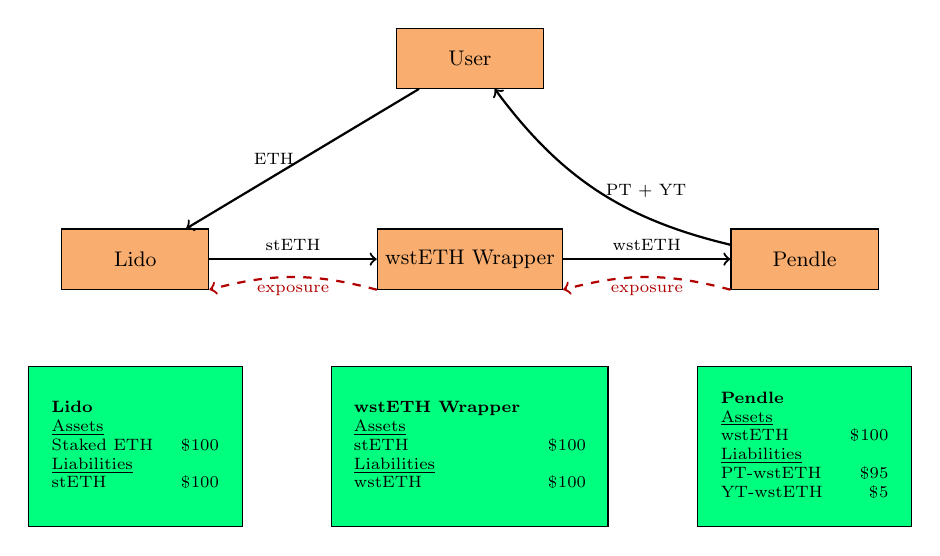
\begin{tikzpicture}[node distance=2.5cm, auto, scale=0.85, transform shape]
        \tikzstyle{entity} = [rectangle, draw, fill=Apricot, minimum width=2.2cm, minimum height=0.9cm, font=\small]
        \tikzstyle{balance} = [rectangle, draw, fill=SpringGreen, minimum width=3.2cm, minimum height=2.4cm, font=\scriptsize]
        \tikzstyle{exposure} = [->, thick, dashed, red!70!black]

        % User at top
        \node[entity] (user) at (0,3) {User};

        % Three protocols in a row
        \node[entity] (lido) at (-5,0) {Lido};
        \node[entity] (wrapper) at (0,0) {wstETH Wrapper};
        \node[entity] (pendle) at (5,0) {Pendle};

        % Balance sheets below each protocol
        \node[balance] (balanceLido) at (-5,-2.8) {
            \begin{tabular}{lr}
                \textbf{Lido} & \\
                \underline{Assets} & \\
                Staked ETH & \$100 \\
                \underline{Liabilities} & \\
                stETH & \$100
            \end{tabular}
        };
        \node[balance] (balanceWrapper) at (0,-2.8) {
            \begin{tabular}{lr}
                \textbf{wstETH Wrapper} & \\
                \underline{Assets} & \\
                stETH & \$100 \\
                \underline{Liabilities} & \\
                wstETH & \$100
            \end{tabular}
        };
        \node[balance] (balancePendle) at (5,-2.8) {
            \begin{tabular}{lr}
                \textbf{Pendle} & \\
                \underline{Assets} & \\
                wstETH & \$100 \\
                \underline{Liabilities} & \\
                PT-wstETH & \$95 \\
                YT-wstETH & \$5
            \end{tabular}
        };

        % Token flows (solid arrows)
        \draw[->, thick] (user) -- node[left, font=\scriptsize] {ETH} (lido);
        \draw[->, thick] (lido) -- node[above, font=\scriptsize] {stETH} (wrapper);
        \draw[->, thick] (wrapper) -- node[above, font=\scriptsize] {wstETH} (pendle);
        \draw[->, thick] (pendle) to[bend left=20] node[right, font=\scriptsize] {PT + YT} (user);

        % Credit exposure arrows (dashed red)
        \draw[exposure] (pendle.south west) to[bend right=15] node[below, font=\scriptsize, text=red!70!black] {exposure} (wrapper.south east);
        \draw[exposure] (wrapper.south west) to[bend right=15] node[below, font=\scriptsize, text=red!70!black] {exposure} (lido.south east);

    \end{tikzpicture}
    \caption{Multi-layer credit exposure in DeFi. A user stakes ETH with Lido, receiving stETH, which is wrapped into wstETH and deposited into Pendle. Each protocol holds the liability of the preceding one, creating a chain of credit exposures from Pendle to Lido.}
    \label{fig:exposure_example}
\end{figure}

\noindent Figure~\ref{fig:exposure_example} illustrates how a single user transaction creates a multi-layer chain of credit exposures in DeFi.  A user deposits ETH into Lido, a liquid staking protocol, and receives stETH, a rebasing token that accrues staking rewards.  The stETH is then wrapped into wstETH, a non-rebasing representation that is more compatible with DeFi protocols.  Finally, wstETH is deposited into Pendle, a yield-tokenisation protocol that splits the asset into a principal token PT-wstETH and a yield token YT-wstETH, allowing users to trade fixed and variable yield separately.

In balance-sheet terms, Lido holds staked ETH with validators and issues stETH as liabilities, the wstETH wrapper holds stETH and issues wstETH, and Pendle holds wstETH and issues the PT and YT pair.  Because each protocol's assets consist of tokens issued by the preceding protocol, a chain of credit exposures emerges: Pendle has exposure to the wstETH wrapper, which in turn has exposure to Lido.  If Lido experienced a slashing event or stETH de-pegged from ETH, the losses would cascade through wstETH and into Pendle, affecting PT and YT holders.  This example demonstrates that DeFi exposures are inherently multi-layered, as liquid staking, wrapping, and yield tokenisation compound into complex dependency structures that the DeXposure dataset aims to capture.

\subsection{Mapping Tokens to Issuing Protocols}

To operationalise \eqref{eq:credit-exposure-definition}, we must determine which protocol issues each token and thus identify the direction of exposure.  Let $\mathcal{P}$ denote the set of all protocols and $\mathcal{C}$ the set of blockchains.  For each token $\sigma$ appearing in protocol $p$, a \textbf{mapping function} $M(\sigma)$ returns the protocol $q$ that issues or manages $\sigma$.  The DeXposure dataset constructs $M$ using a fall‑back procedure:
\begin{enumerate}
  \item \textbf{Metadata lookup:} Tokens are directly matched to issuing protocols using metadata from DefiLlama when available.
  \item \textbf{Manual mapping:} For tokens with high TVL that lack metadata links, researchers manually assign the issuing protocol based on documentation and expert knowledge.
  \item \textbf{Text‑vector similarity:} For remaining tokens, the text descriptions of tokens and protocols are vectorised via the term frequency–inverse document frequency (TF--IDF) representation \cite{Qaiser2018}.  Cosine similarity scores between token and protocol vectors determine the best match, and tokens are mapped to the protocol with the highest similarity score exceeding a threshold $\theta$.
  \item \textbf{Primary market tokens:} If none of the above methods yields a mapping, the token is treated as its own protocol (e.g., WETH).
\end{enumerate}
This mapping ensures that token flows between protocols can be attributed to changes in credit exposure with respect to the correct issuing protocol, even when tokens are bridged across chains or wrapped by multiple platforms.

\subsection{Network Representation and Value Flows}

Credit exposures over a discrete time interval $\tau = t_2 - t_1$ are represented by a weighted directed graph $G_\tau = (P_\tau, E_\tau)$, where $P_\tau$ is the set of active protocols and $E_\tau$ is the set of directed edges.  Each vertex $p\in P_\tau$ is assigned a \textbf{node weight} equal to the value of assets it holds at the end of the interval:
\begin{equation}
w_\tau(p) = \sum_{\sigma\in X_p(t_1)\cap X_p(t_2)} v_{t_2,\sigma},
\label{eq:node-weight}
\end{equation}
where $v_{t_2,\sigma}$ is the USD value of token $\sigma$ at time $t_2$.  Nodes with negligible weight (below a threshold $\theta$) can be pruned for clarity.  To define the \textbf{edge weight} from protocol $p$ to protocol $q$, we first compute the value flow for each token $\sigma$:
\begin{equation}
F^{\sigma}_{p q,\tau} =
\begin{cases}
\max\bigl(0,\, -\Delta S^{\sigma}_{p,\tau}\bigr), & \text{if } \Delta S^{\sigma}_{p,\tau} < 0,\\
\max\bigl(0,\,\Delta S^{\sigma}_{q,\tau}\bigr), & \text{if } \Delta S^{\sigma}_{q,\tau} \ge 0,
\end{cases}
\label{eq:value-flow}
\end{equation}
where $\Delta S^{\sigma}_{p,\tau}=v_{p,t_2}^{\sigma}-v_{p,t_1}^{\sigma}$ is the change in the USD value of token $\sigma$ held by protocol $p$ over the interval.  Equation~\eqref{eq:value-flow} captures the intuition that if $p$ decreases its holdings of $\sigma$ and $q$ increases theirs, then $\sigma$ has flowed from $p$ to $q$; negative flows are reversed so that all flows are non‑negative.  The \textbf{edge weight} $w_\tau(e_{p q})$ is the sum of flows for all tokens that map to the issuing protocol $q$:
\begin{equation}
w_\tau(e_{p q}) = \sum_{\sigma \in X_{p q, \tau}} F^{\sigma}_{p q,\tau},
\label{eq:edge-weight}
\end{equation}
where $X_{p q,\tau}$ denotes the set of tokens with issuing protocol $q$ that move from $p$ to $q$ over $\tau$.  A positive edge weight indicates increasing exposure from $p$ to $q$.  For single‑token protocols, the flow of that token equals the edge weight.

Algorithm~1 in \cite{wu2025} describes a procedure for constructing $G_\tau$ from raw token‑protocol‑chain mappings.  In summary, one aggregates token holdings at the start and end of the interval, computes node weights, discards nodes below a threshold, and then computes edge weights by summing positive flows; negative flows are reversed to ensure all weights are non‑negative.  The resulting time‑indexed sequence of graphs captures the evolving structure of credit dependencies in the DeFi ecosystem.

\subsection{Discussion and links to systemic‑risk theory}

The above formalism bridges decentralised finance with established theories of financial networks.  By modelling credit exposures as weighted directed graphs derived from token flows, it becomes possible to apply systemic‑risk measures, such as centrality metrics, contagion indices, and stress tests, developed for interbank networks to DeFi.  Classical models show that fixed‑point algorithms can compute consistent clearing payments for interbank systems with cyclic obligations \cite{EisenbergNoe2001}, and that network structures can either buffer or amplify shocks depending on leverage and liquidity \cite{Glasserman2016}.  \cite{Acemoglu2013} further demonstrate that more complete networks initially enhance stability by distributing losses across many counterparties, but beyond a critical density the same interconnections propagate shocks and increase systemic fragility.  In the DeFi context, our graph formalisation reveals similar trade‑offs: diversifying collateral across multiple protocols may reduce reliance on any single issuer, yet highly interconnected protocols could become conduits for contagion if a stablecoin or wrapped token suffers a de‑peg or exploit.

This mathematical framework provides the foundation for the downstream tasks tackled by DeXposure‑FM.  Forecasting future node and edge weights, stress‑testing scenarios under shocks to token values, and imputing missing TVL data all rely on accurate representations of credit exposure.  Moreover, the network perspective aligns with macroprudential policy goals: regulators can monitor systemic importance and spillover risks by examining the temporal evolution of $G_\tau$, and researchers can evaluate how proposed protocol designs or regulatory interventions would reshape the exposure network.  As decentralised finance continues to grow and integrate with the broader financial system, rigorous formalisation and measurement of credit exposure will be essential for safeguarding stability and fostering responsible innovation.
\section{DeXposure-FM: Architecture, Data, and Training}

This section introduces our DeXposure-FM, including its architecture, preparation of data, and the training process. The code is available at \url{https://github.com/EVIEHub/DeXposure-FM}.


\subsection{Model Architecture}\label{subsec:model-arch}

DeXposure-FM is a time-series graph foundation model designed to forecast the evolution of inter-protocol credit exposures. The architecture follows an \emph{encoder-multi-head} design: a pretrained graph-tabular encoder produces protocol embeddings for each weekly snapshot, and then multiple heads map these embeddings to (1) edge existence and exposure changes, (2) node-level TVL dynamics, and (3) induced network statistics.

\subsubsection{Input and Features}
Let $t\in\mathcal{T}$ be discrete observation times and $\tau=(t_1,t_2)$ be a weekly interval. For each $\tau$, we construct a weighted directed exposure graph
\begin{equation}
G_\tau=(\mathcal{P}_\tau,\mathcal{E}_\tau),
\end{equation}
where nodes $p\in\mathcal{P}_\tau$ are protocols and edges $(p,q)\in\mathcal{E}_\tau$ represent token-mediated exposure from $p$ to issuing protocol $q$. Node weights encode protocol size (TVL) and edge weights encode the weekly change in exposure induced by token flows and valuation updates. Each node $p$ additionally has a tabular descriptor vector $ x^{\text{tab}}_{p,\tau}$ including log-scaled TVL and token-composition summaries (e.g., number of token types held, concentration measures, entropy) and a sector/category one-hot encoding.

\subsubsection{Pretrained Graph-Tabular Encoder}

We adopt {GraphPFN} as the encoder $E(\cdot)$ in our model, which is a transformer-based graph-tabular foundation model that fuses graph structure with tabular node features via multi-head self-attention augmented with structural information \citep{eremeev2025turningtabularfoundationmodels}. Given $(G_\tau,\{ x^{\text{tab}}_{p,\tau}\}_{p\in\mathcal{P}_\tau})$, the encoder produces
$d$-dimensional node representations
\begin{equation}
\{h_{p,\tau}\}_{p\in\mathcal{P}_\tau}
= E_{\text{GraphPFN}}\!\left(G_\tau,\{ x^{\text{tab}}_{p,\tau}\}_{p\in\mathcal{P}_\tau}\right),
\qquad h_{p,\tau}\in\mathbb{R}^d .
\end{equation}

\subsubsection{Edge-Level Prediction Head}

For each forecast horizon $h\in\{1, 4, 8, 12\}$ weeks, DeXposure-FM predicts both edge existence and edge weight (i.e., exposure change) for ordered protocol pairs $(p,q)$. We form a pairwise feature vector using a standard symmetric composition of embeddings:
\begin{equation}
 f_{pq,\tau}=\Big[ h_{p,\tau};\,  h_{q,\tau};\,  h_{p,\tau}\odot   h_{q,\tau};\,\lvert  h_{p,\tau}-  h_{q,\tau}\rvert\Big],
\end{equation}
and pass it through a multi-layer perceptron (MLP) head to obtain
\begin{equation}
(\widehat{y}^{\mathrm{exist}}_{pq}, \widehat{w}_{\tau+h}(e_{pq})) = \mathrm{MLP}_{\mathrm{link}}({f}_{pq}),
\end{equation}
where $\widehat{y}^{\mathrm{exist}}_{pq}\in(0,1)$ is the predicted probability of edge existence, and $\widehat{w}_{\tau+h}(e_{pq})$ is the predicted edge weight (log-scaled).

\subsubsection{Node-Level Prediction Head and Network Statistics}

To capture protocol-level dynamics, we predict the log-change in protocol TVL using a node head:
\begin{align*}
    \widehat{\Delta}_{p,\tau+h} = &\mathrm{MLP}_{\mathrm{node}}({h}_{p,\tau}),\\
\widehat{\Delta}_{p,\tau+h} =& \log(1+w_{\tau+h}(p)) - \log(1+w_{\tau}(p)),
\end{align*}
for protocols $p\in\mathcal{P}_{\tau}\cap\mathcal{P}_{\tau+h}$.

Network-level statistics (e.g., density, concentration measures, and sector connectivity) are computed as deterministic functionals of the predicted graph $\widehat{G}_{\tau+h}$, enabling evaluation of the model both at the edge level and at the level of aggregate stability indicators.


\subsection{Training Pipeline}\label{subsec:training-pipeline}

This section describes how we construct supervised training pairs from weekly DeXposure snapshots, define the multi-task learning objective, and optimize DeXposure-FM.

\subsubsection{Data Preparation}\label{subsubsec:data-prep}
DeXposure provides weekly snapshots of the inter-protocol exposure network. For each discrete time index $\tau$, we construct a weighted directed graph
$G_{\tau}=(\mathcal{P}_{\tau},\mathcal{E}_{\tau})$ with node weights $w_{\tau}(p)$ (protocol TVL) and edge weights $w_{\tau}(e_{pq})$ (exposure from $p$ to $q$).
Training examples are formed by an \emph{anchor} snapshot and a forecast horizon:
\begin{equation}
G_{\tau} \;\longrightarrow\; G_{\tau+h},
\qquad
h\in\{1,4,8,12\},
\label{eq:train-pairs}
\end{equation}
so that the model predicts the future graph state at horizon $h$ conditional on the current snapshot.

For each protocol $p\in\mathcal{P}_{\tau}$ we provide tabular node features $x^{\text{tab}}_{p,\tau}$ (including log-scaled TVL, token counts, concentration measures, and sector/category indicators) together with the graph structure $G_{\tau}$.

Table~\ref{tab:data-stats} summarizes the dataset characteristics. The network exhibits high edge persistence (mean overlap ratio 98.5\%), reflecting the stable nature of DeFi protocol interconnections.

\begin{table}[t]
\centering
\small
\begin{tabular}{lr}
\hline
\textbf{Statistic} & \textbf{Value} \\
\hline
Total snapshots & 283 weeks \\
Time range & 2020-03-23 $\sim$ 2025-08-18 \\
Mean nodes per week & 5,676 \\
Mean edges per week & 30,424 \\
Mean edge overlap ratio & 98.5\% \\
Protocol categories & $\sim$ \\
\hline
\end{tabular}
\caption{DeXposure dataset statistics.}
\label{tab:data-stats}
\end{table}

\textbf{Time-based expanding window splits.}
We adopt an expanding-window walk-forward evaluation protocol to prevent look-ahead bias: all validation and test targets occur strictly after the corresponding training window, and the training window expands over time while validation and test windows remain fixed.

\textbf{Negative sampling.}
Edge existence is highly imbalanced.  For each horizon $h$, we construct a labeled edge set $\mathcal{S}_{\tau+h}$ consisting of all positive edges in $\mathcal{E}_{\tau+h}$ plus uniformly sampled negative edges from the complement, using a negative-to-positive ratio of $5{:}1$.
This sampled set is used for the edge existence loss, while the edge weight loss is computed only on positive edges.

\subsubsection{Loss Functions}\label{subsubsec:loss}
DeXposure-FM is trained with a multi-task objective combining (1) edge existence classification, (2) edge weight regression, and (3) node-level TVL-change prediction.

\textbf{Edge existence (link prediction).}
For each candidate pair $(p,q)\in\mathcal{S}_{\tau+h}$ we predict $\widehat{y}^{\text{exist}}_{pq}\in(0,1)$ and minimize a weighted binary cross-entropy loss:
\begin{equation}
\mathcal{L}_{\text{exist}}
=
\sum_{(p,q)\in\mathcal{S}_{\tau+h}}
\mathrm{BCE}\!\left(\widehat{y}^{\text{exist}}_{pq},\,y^{\text{exist}}_{pq};\,w_{\text{pos}}\right),
\label{eq:loss-exist}
\end{equation}
where $w_{\text{pos}}$ upweights positives to match the negative sampling ratio. Here, binary cross-entropy is defined as below. 

\begin{definition}[binary cross-entropy (BCE)]
For a binary label $y\in\{0,1\}$ and a predicted probability $\hat{y}\in(0,1)$, the binary cross-entropy loss is
\begin{equation}
\mathrm{BCE}(\hat{y},y)
= -\Big(y\log(\hat{y}) + (1-y)\log\big(1-\hat{y}\big)\Big).
\label{eq:bce}
\end{equation}
Equivalently, if $\hat{y}=\sigma(z)$ is produced from a logit $z\in\mathbb{R}$ via the sigmoid $\sigma(z)=1/(1+e^{-z})$, then
\begin{equation}
\mathrm{BCE}(\sigma(z),y)
= \log\!\big(1+e^{z}\big) - yz,
\label{eq:bce-logit}
\end{equation}
which is numerically stable and is often referred to as the logistic loss.
\end{definition}

\textbf{Edge weights (residual learning).}
For positive edges $(p,q)\in\mathcal{E}_{\tau+h}$ we predict a residual in log space relative to the previous observed week. Let $\tilde{w}_{\tau}(e_{pq})=\log(1+w_{\tau}(e_{pq}))$ and $\tilde{w}_{\tau+h}(e_{pq})=\log(1+w_{\tau+h}(e_{pq}))$. The link head outputs $\widehat{r}_{pq,\tau,h}$ and we apply a robust Smooth~L1 loss:
\begin{equation}
\mathcal{L}_{\text{weight}}
=
\sum_{(p,q)\in\mathcal{E}_{\tau+h}}
\mathrm{SmoothL1}\!\Big(
\widehat{r}_{pq,\tau,h}
-
\big(\tilde{w}_{\tau+h}(e_{pq})-\tilde{w}_{\tau}(e_{pq})\big)
\Big).
\label{eq:loss-weight}
\end{equation}
Equivalently, we reconstruct $\widehat{\tilde{w}}_{\tau+h}(e_{pq})=\tilde{w}_{\tau}(e_{pq})+\widehat{r}_{pq,\tau,h}$ and minimize $\mathrm{SmoothL1}(\widehat{\tilde{w}}_{\tau+h}(e_{pq})-\tilde{w}_{\tau+h}(e_{pq}))$. We set $\tilde{w}_{\tau}(e_{pq})=0$ when the edge is absent at time $\tau$. The $\log(1+\cdot)$ transform stabilizes training under the heavy-tailed exposure distribution. Here, smooth L1 (Huber) loss is defined as follows.
\begin{definition}[smooth L1 (Huber) loss]
For a scalar prediction $\hat{u}\in\mathbb{R}$ and target $u\in\mathbb{R}$, let the residual be $r=\hat{u}-u$.
The Smooth~L1 (Huber) loss with threshold $\delta>0$ is defined as
\begin{equation}
\mathrm{SmoothL1}_\delta(r)=
\begin{cases}
\frac{1}{2}\frac{r^2}{\delta}, & \text{if } |r|<\delta,\\[6pt]
|r|-\frac{1}{2}\delta, & \text{otherwise}.
\end{cases}
\label{eq:smoothl1}
\end{equation}
Equivalently, written directly in terms of $(\hat{u},u)$:
\begin{equation}
\mathrm{SmoothL1}_\delta(\hat{u},u)=
\begin{cases}
\frac{1}{2}\frac{(\hat{u}-u)^2}{\delta}, & \text{if } |\hat{u}-u|<\delta,\\[6pt]
|\hat{u}-u|-\frac{1}{2}\delta, & \text{otherwise}.
\end{cases}
\end{equation}
\end{definition}
Smooth~L1 behaves like an $\ell_2$ loss near zero (encouraging small residuals) and like an $\ell_1$ loss for large residuals (reducing sensitivity to heavy tails and outliers). A common choice is $\delta=1$, when $\mathrm{SmoothL1}_\delta$ is briefly written as $\mathrm{SmoothL1}$.

\textbf{Node-level TVL dynamics.}
We also predict the log-change in protocol TVL,
$\Delta_{p,\tau+h}=\log(1+w_{\tau+h}(p))-\log(1+w_{\tau}(p))$,
using Smooth~L1:
\begin{equation}
\mathcal{L}_{\text{node}}
=
\sum_{p\in\mathcal{P}_{\tau}\cap \mathcal{P}_{\tau+h}}
\mathrm{SmoothL1}\!\left(\widehat{\Delta}_{p,\tau+h}-\Delta_{p,\tau+h}\right),
\label{eq:loss-node}
\end{equation}
where $\Delta_{p,\tau+h} = \log(1+w_{\tau+h}(p)) - \log(1+w_{\tau}(p))$ is the ground-truth log-change in TVL.


\textbf{Multi-task objective.}
The total loss is a weighted sum:
\begin{equation}
\mathcal{L}
=
\lambda_{\text{exist}}\mathcal{L}_{\text{exist}}
+
\lambda_{\text{weight}}\mathcal{L}_{\text{weight}}
+
\lambda_{\text{node}}\mathcal{L}_{\text{node}},
\label{eq:loss-total}
\end{equation}
with $\lambda_{\text{exist}}=2.0$, $\lambda_{\text{weight}}=0.5$, and $\lambda_{\text{node}}=20.0$. These weights are calibrated to balance the gradient contributions across tasks despite their different loss magnitudes: edge existence loss $\mathcal{L}_{\mathrm{exist}} \approx 0.22$, edge weight loss $\mathcal{L}_{\mathrm{weight}} \approx 2.4$, and node loss $\mathcal{L}_{\mathrm{node}} \approx 0.05$ on average. They also reflect the primary importance of link prediction while using weight and node supervision to encourage economically meaningful representations. 

\subsubsection{Optimization}\label{subsubsec:optim}

\textbf{Initialization.} We adopt the open-source weights of GraphPFN as initialization of the encoder. 

\textbf{Optimizer.}
We use Adam \citep{KingmaBa2015Adam} with hyperparameters $\beta_1=0.9$, $\beta_2=0.999$ and learning rate $\eta = 5 \times 10^{-4}$.

\textbf{Training details.}
We train for up to 20 epochs with early stopping (patience = 3) based on validation AUPRC. Gradient clipping ($\|\nabla\|_2 \le 1.0$) is applied for stability.


\textbf{Optional sharpness-aware training.}
Sharpness-Aware Minimization (SAM) is a promising extension to improve robustness under non-stationarity by favoring flatter optima. However, our current released training pipeline and the experiments reported in this paper use Adam; we leave SAM-based training as future work.

\begin{table}[t]
\centering
\small
\setlength{\tabcolsep}{6pt}
\renewcommand{\arraystretch}{1.05}
\begin{tabular}{ll}
\hline
\textbf{Hyperparameter} & \textbf{Value} \\
\hline
Data granularity & Weekly snapshots \\
Forecast horizons $h$ & $\{1, 4, 8, 12\}$ weeks \\
Negative sampling ratio & 5:1 (neg:pos) \\
Optimizer & Adam ($\beta_1=0.9$, $\beta_2=0.999$) \\
Learning rate (heads) & $5 \times 10^{-4}$ \\
Learning rate (backbone) & $5 \times 10^{-5}$ (fine-tune only) \\
Training epochs & 20 (early stopping patience=3) \\
Gradient clipping & $\|\nabla\|_2 \le 1.0$ \\
\hline
\multicolumn{2}{l}{\textit{Loss weights:}} \\
$\lambda_{\mathrm{exist}}$ (edge existence) & $2.0$ \\
$\lambda_{\mathrm{weight}}$ (edge weight) & $0.5$ \\
$\lambda_{\mathrm{node}}$ (node prediction) & $20.0$ \\
\hline
\end{tabular}
\caption{Training hyperparameters for DeXposure-FM experiments.}
\label{tab:training-hparams}
\end{table}

\noindent Empirical evaluations on machine-learning benchmarks are reported in Section~\ref{sec:evaluation}, and financial-economics tools and case-study verifications are presented in Section~\ref{sec:econ}.


\begin{comment}
    
\newpage

\section{Empirical Evaluations on Machine Learning Benchmarks}

\subsection{Task 1:  Multi-step Forecasting}

\textbf{Implementation Deatails}

\textbf{Empirical Results}

\subsection{Task 2: xx}

\textbf{Implementation Deatails}

\textbf{Empirical Results}

\section{Financial Economics Tools and Experimental Verifications}

\subsection{Macroprudential Applications}

\textbf{Systemic importance ranking.}

\textbf{Sector spillover monitoring. }

\textbf{Stress testing and contagion assessment.}

\textbf{Early warning signals.}

\subsection{Validity and Scope}
\end{comment}


\section{Empirical Evaluations on Machine Learning Benchmarks}
\label{sec:evaluation}

We evaluate DeXposure-FM on the DeXposure dataset through two machine learning benchmark tasks: (i) \textit{multi-step forecasting} of edge existence/weights and node TVL changes; and (ii) \textit{predictive contagion stress testing}, where we forecast future stress-test losses under counterfactual shocks. Section~\ref{sec:econ} then translates these predictive outputs into macroprudential monitoring tools (systemic importance, spillovers, stress testing, and early warning) and validates them on historical stress events.

\subsection{Dataset and Experimental Setup}
\label{subsec:dataset}

\paragraph{Data source.}
We use the DeXposure dataset constructed from DeFiLlama API data, spanning March 2020 to August 2025 (283 weekly snapshots). Each snapshot contains protocol nodes with TVL measurements and directed edges representing credit exposures between protocols.

\paragraph{Data statistics.}
Table~\ref{tab:data-stats} summarizes the dataset characteristics. The network exhibits high edge persistence (mean overlap ratio 98.5\%), reflecting the stable nature of DeFi protocol interconnections.

\begin{table}[t]
\centering
\small
\begin{tabular}{lr}
\hline
\textbf{Statistic} & \textbf{Value} \\
\hline
Total snapshots & 283 weeks \\
Time range & 2020-03-23 $\sim$ 2025-08-18 \\
Mean nodes per week & 5,676 \\
Mean edges per week & 30,424 \\
Mean edge overlap ratio & 98.5\% \\
Protocol categories & $\sim$15 classes \\
\hline
\end{tabular}
\caption{DeXposure dataset statistics.}
\label{tab:data-stats}
\end{table}

\paragraph{Temporal split.}
We use a two-stage evaluation protocol:

\textit{Stage 1: Model selection via walk-forward cross-validation.}
We apply expanding window walk-forward cross-validation on pre-2025 data with 15 folds. Each fold uses a minimum of 104 training weeks, 24 validation weeks (for early stopping), and 8 test weeks. The validation window is sized to ensure sufficient samples even at longer horizons: for $h=12$, we require $\geq 12$ validation weeks to construct valid forecast pairs. The window advances by 8 weeks per fold, accumulating more training data. This stage is used for hyperparameter selection and model comparison.

\textit{Stage 2: Hold-out evaluation.}
Final performance is reported on a strict 2025 hold-out set, which is never seen during training or validation:
\begin{itemize}
  \item \textbf{Training:} 2020-03-23 $\sim$ 2024-07-15 (225 weeks)
  \item \textbf{Validation:} 2024-07-22 $\sim$ 2024-12-30 (24 weeks, for early stopping)
  \item \textbf{Test:} 2025-01-06 $\sim$ 2025-08-18 (33 weeks, strict hold-out)
\end{itemize}
Stage 1 is used for hyperparameter tuning; all results reported in this paper are from Stage 2 hold-out evaluation.

\paragraph{Forecast horizons vs. CV windows.}
The 8-week CV window controls how the temporal folds slide; within each window, the model predicts at multiple forecast horizons $h \in \{1, 4, 8, 12\}$ weeks ahead. These are orthogonal: the CV window determines sample collection, while $h$ determines how far into the future each prediction extends.

\paragraph{Models compared.}
We compare three approaches:
\begin{enumerate}
  \item \textbf{GraphPFN:} Pre-trained GraphPFN encoder with frozen weights; only task-specific prediction heads are trained (linear probe).
  \item \textbf{DeXposure-FM:} Pre-trained GraphPFN encoder with end-to-end fine-tuning using differential learning rates.
\item \textbf{ROLAND:} Representative temporal GNN baseline with a 2-layer GCN encoder (hidden\_dim=64, out\_dim=32) and GRU temporal updates for recurrent state propagation, trained from scratch. Uses the same optimizer (Adam), learning rate ($5 \times 10^{-4}$), and training schedule as DeXposure-FM.
\end{enumerate}

\subsection{Task I: Multi-step Forecasting}
\label{subsec:forecast}

\subsubsection{Implementation Details}
\label{subsubsec:task1-impl}
We evaluate forecasts at horizons $h \in \{1, 4, 8, 12\}$ weeks for:
\begin{enumerate}
  \item \textbf{Edge existence:} Binary prediction of whether edge $(p,q)$ exists at $t+h$.
  \item \textbf{Edge weight:} Regression on log-scaled edge weight for existing edges.
  \item \textbf{Node TVL change:} Regression on $\Delta_{p,t+h} = \log(1+\text{TVL}_{t+h}) - \log(1+\text{TVL}_t)$.
\end{enumerate}

\noindent We report AUPRC/AUROC for edge existence and MAE/RMSE for edge weights and node $\Delta$TVL on log-scaled values.

\subsubsection{Empirical Results}
\label{subsubsec:task1-results}
For edge existence, we report AUPRC (area under precision-recall curve) and AUROC. For edge weight and node predictions, we report MAE and RMSE on log-scaled values.

Table~\ref{tab:main-results} presents the main forecasting results on the 2025 hold-out test set.
%% [Updated to h={1,4,8,12} with complete DeXposure-FM results from GPU server experiments]

\begin{table}[t]
\centering
\small
\setlength{\tabcolsep}{4pt}
\begin{tabular}{llcccccc}
\hline
& & \multicolumn{2}{c}{\textbf{Edge Exist}} & \multicolumn{2}{c}{\textbf{Edge Weight}} & \multicolumn{2}{c}{\textbf{Node $\Delta$TVL}} \\
\textbf{Model} & $h$ & AUROC & AUPRC & MAE & RMSE & MAE & RMSE \\
\hline
\multirow{4}{*}{DeXposure-FM}
& 1 & \textbf{0.995} & \textbf{0.972} & \textbf{2.465} & \textbf{3.388} & \textbf{0.056} & \textbf{0.400} \\
& 4 & \textbf{0.995} & \textbf{0.973} & \textbf{2.489} & \textbf{3.424} & \textbf{0.140} & \textbf{0.680} \\
& 8 & \textbf{0.994} & \textbf{0.967} & \textbf{2.554} & \textbf{3.509} & \textbf{0.229} & \textbf{0.890} \\
& 12 & \textbf{0.993} & \textbf{0.967} & \textbf{2.648} & \textbf{3.606} & \textbf{0.286} & \textbf{1.046} \\
\hline
\multirow{4}{*}{GraphPFN}
& 1 & 0.988 & 0.938 & 3.260 & 4.383 & 0.059 & 0.401 \\
& 4 & 0.988 & 0.940 & 3.189 & 4.049 & 0.142 & 0.682 \\
& 8 & 0.987 & 0.938 & 3.169 & 4.064 & 0.215 & 0.896 \\
& 12 & 0.986 & 0.936 & 3.136 & 4.130 & 0.324 & 1.056 \\
\hline
\multirow{4}{*}{ROLAND}
& 1 & 0.961 & 0.865 & 3.240 & 4.264 & 0.060 & 0.403 \\
& 4 & 0.962 & 0.868 & 3.242 & 4.162 & 0.141 & 0.684 \\
& 8 & 0.961 & 0.867 & 3.213 & 4.180 & 0.221 & 0.895 \\
& 12 & 0.961 & 0.866 & 3.195 & 4.177 & 0.279 & 1.058 \\
\hline
\multirow{4}{*}{Persistence}
& 1 & 0.763 & 0.604 & 2.487 & 4.296 & 0.057 & 0.403 \\
& 4 & 0.782 & 0.635 & 2.372 & 4.138 & 0.138 & 0.685 \\
& 8 & 0.749 & 0.580 & 2.618 & 4.400 & 0.213 & 0.899 \\
& 12 & 0.762 & 0.603 & 2.541 & 4.304 & 0.272 & 1.065 \\
\hline
\end{tabular}
\caption{Multi-step forecasting results on 2025 hold-out test set at horizons $h \in \{1,4,8,12\}$ weeks. DeXposure-FM = Finetuned Foundation Model, GraphPFN = Graph Prior Fitted Network with Frozen weights. \textit{Persistence} = naive baseline predicting $\hat{A}_{t+h} = A_t$, $\hat{W}_{t+h} = W_t$.}
\label{tab:main-results}
\end{table}

\paragraph{Key findings.}
\begin{enumerate}
  \item \textbf{Edge existence substantially exceeds persistence:} All models dramatically outperform the naive persistence baseline (AUPRC 0.58--0.64) that simply predicts ``last week's graph.'' DeXposure-FM achieves AUPRC 0.967--0.973, representing a 52--67\% relative improvement over persistence. This confirms the models learn meaningful temporal dynamics beyond network inertia.
  \item \textbf{Edge weight matches persistence:} Surprisingly, edge weight prediction shows no improvement over the persistence baseline (MAE 2.37--2.62). DeXposure-FM achieves MAE 2.465--2.648, comparable to or slightly worse than persistence at some horizons. This indicates that learned models excel at predicting \textit{which} edges exist, but predicting \textit{how much} exposure flows through them remains fundamentally challenging---the best strategy is often ``predict last week's value.''
  \item \textbf{Model value is in link prediction:} The primary value of DeXposure-FM lies in edge existence prediction. Compared to learned baselines, it achieves 3--8\% AUPRC improvement over GraphPFN and 10--12\% over ROLAND, while maintaining comparable weight and node predictions.
  \item \textbf{Node prediction degrades with horizon:} Node TVL change prediction degrades as expected: DeXposure-FM MAE increases from 0.056 ($h=1$) to 0.286 ($h=12$), matching persistence (0.057--0.272) at all horizons.
\end{enumerate}

\subsection{Task II: Financial Stability Analysis}
\label{subsec:stability}

This task evaluates whether forward-looking network forecasts translate into forward-looking \emph{stress test} forecasts. Specifically, we compare contagion losses computed on the model-predicted future network $\hat{G}_{t+h}$ with losses on the realized future network $G_{t+h}$, under fixed counterfactual shock definitions.

\subsubsection{Implementation Details}
\label{subsubsec:task2-impl}
We use a fixed DeXposure-FM forecaster trained on the pre-2025 training period and early-stopped on the pre-2025 validation period (Stage 2 in Section~\ref{subsec:dataset}). We then evaluate on the strict 2025 hold-out set without re-estimation during the test period. Each test week provides an origin $t$, yielding multiple out-of-sample pairs $(t,t+h)$ for horizons $h\in\{1,4,8,12\}$. To handle protocol entry/exit, all comparisons are computed on the common node set $V_t \cap V_{t+h}$.

Stress-test losses are computed using a DebtRank-style contagion simulator (Section~\ref{subsubsec:contagion}) under three scenarios: (i) \textbf{Top protocol shock} (50\% TVL loss to the largest protocol), (ii) \textbf{Top-5 protocols shock} (30\% TVL loss to the top-5 protocols), and (iii) \textbf{Bridge sector shock} (100\% TVL loss to bridge protocols). For each $(t,t+h)$, we run the simulator on three graphs: the observed network at $t$ (persistence baseline), the predicted network $\hat{G}_{t+h}$, and the realized network $G_{t+h}$.

Because the DeFi exposure network is highly persistent (Table~\ref{tab:data-stats}), the persistence baseline is difficult to beat on average. To surface policy-relevant headroom, we also evaluate an \emph{advantage regime}: the \textbf{worst 20\%} of test cases under persistence (largest baseline absolute errors within each horizon, pooled across shock scenarios). We summarize performance with $\Delta \mathrm{MAE}=\mathrm{MAE}(\text{baseline})-\mathrm{MAE}(\text{model})$, where positive values indicate improvement over persistence.

\subsubsection{Empirical Results}
\label{subsubsec:task2-results}
Figure~\ref{fig:contagion-comparison} shows the three-way comparison (baseline vs.\ model vs.\ realized) and Figure~\ref{fig:contagion-advantage} visualizes $\Delta\mathrm{MAE}$ in both the overall population and the worst-20\% tail. Table~\ref{tab:contagion-advantage} reports horizon-level summary statistics.

Across horizons, persistence remains strong on average ($\Delta\mathrm{MAE}(\text{all})<0$), but DeXposure-FM consistently improves performance in the tail ($\Delta\mathrm{MAE}(\text{worst20\%})>0$), with worst20\% win rates of 83--100\%. These gains are concentrated in bridge-sector shocks (Figure~\ref{fig:contagion-advantage}), consistent with non-stationary exposure reallocation through cross-chain liquidity conduits. Section~\ref{sec:econ} further examines how these forecasts support macroprudential tools such as forward-looking risk metric monitoring and early warning event studies.

\begin{figure}[t]
\centering
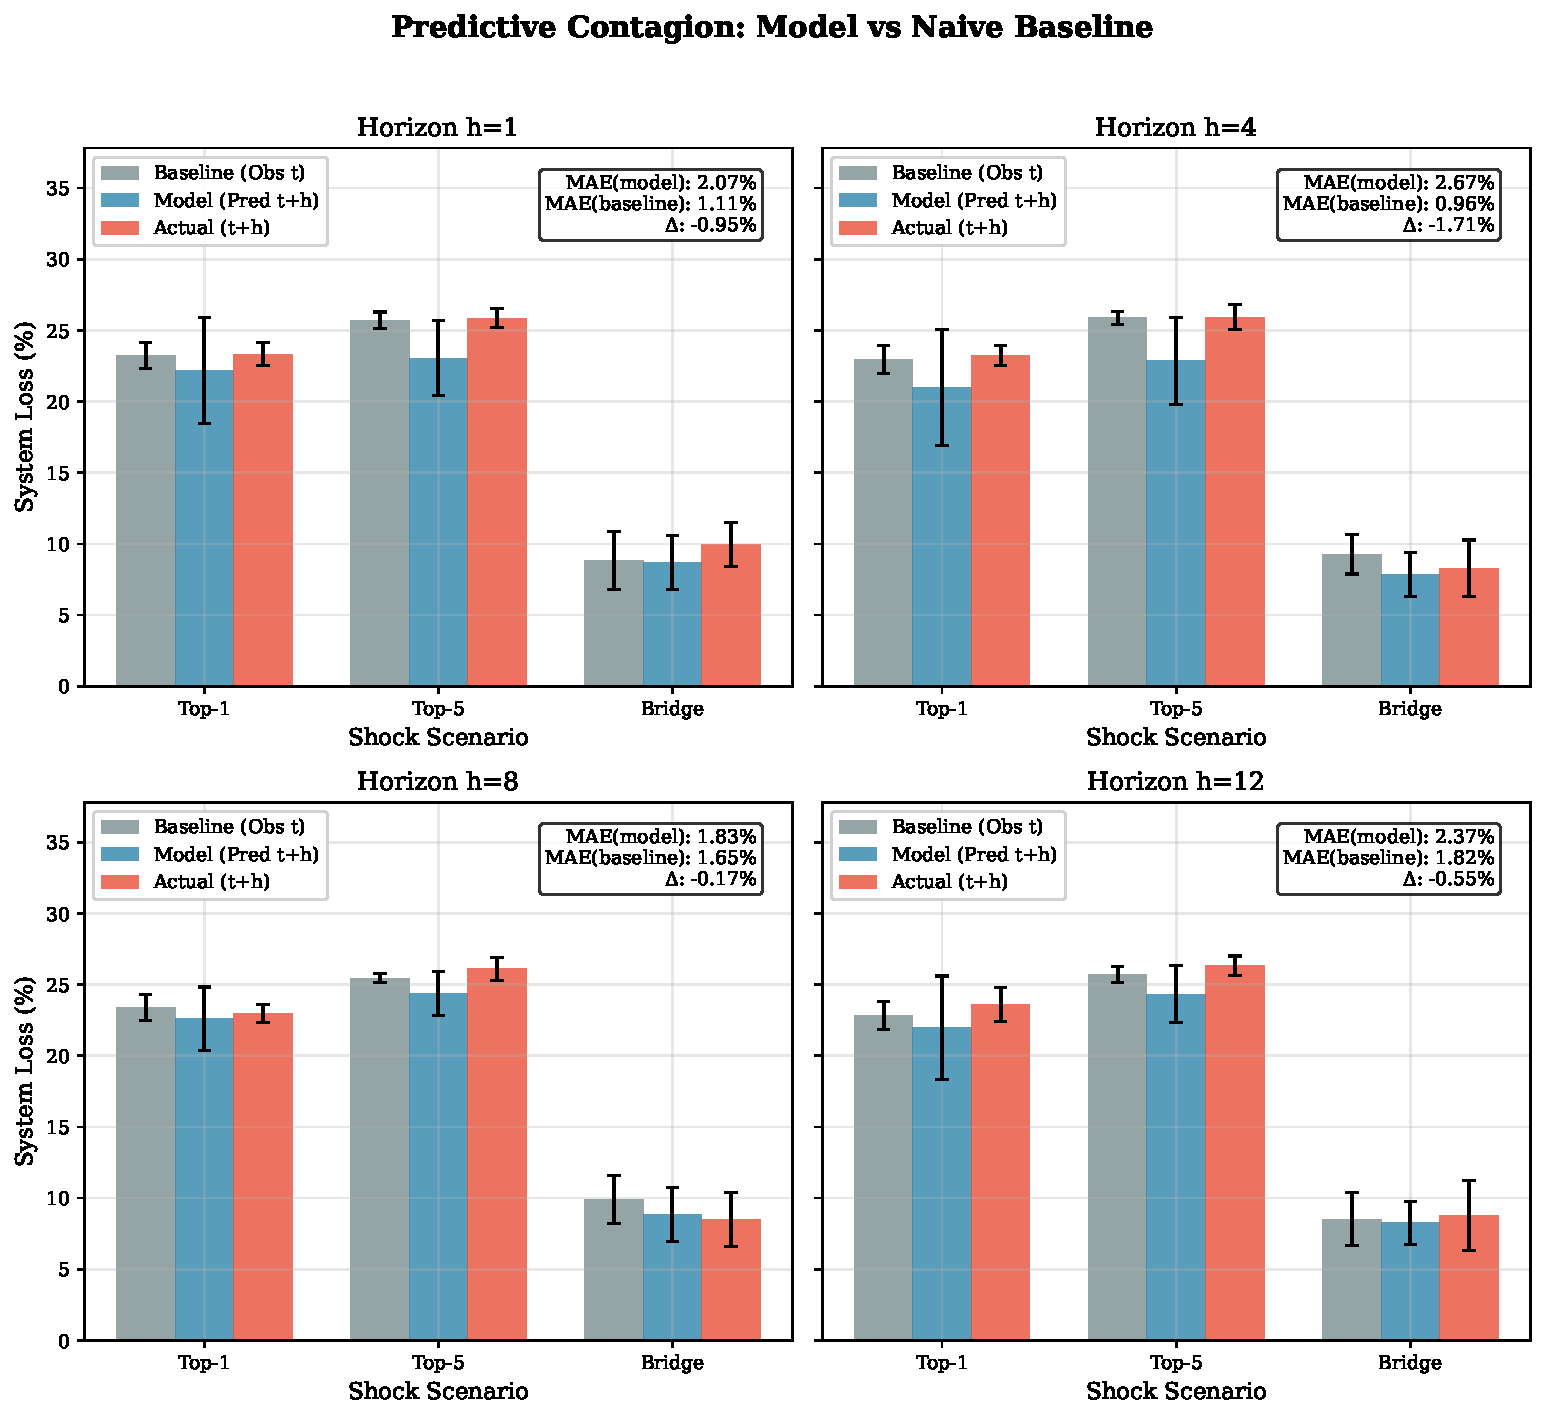
\includegraphics[width=0.95\textwidth]{figures/fig_contagion_comparison.pdf}
\caption{Predictive contagion stress testing (Task II). We compare system loss (\%) under identical shocks when running the contagion simulator on the observed network at time $t$ (persistence baseline), the model-predicted network $\hat{G}_{t+h}$, and the realized future network $G_{t+h}$.}
\label{fig:contagion-comparison}
\end{figure}

\begin{figure}[t]
\centering
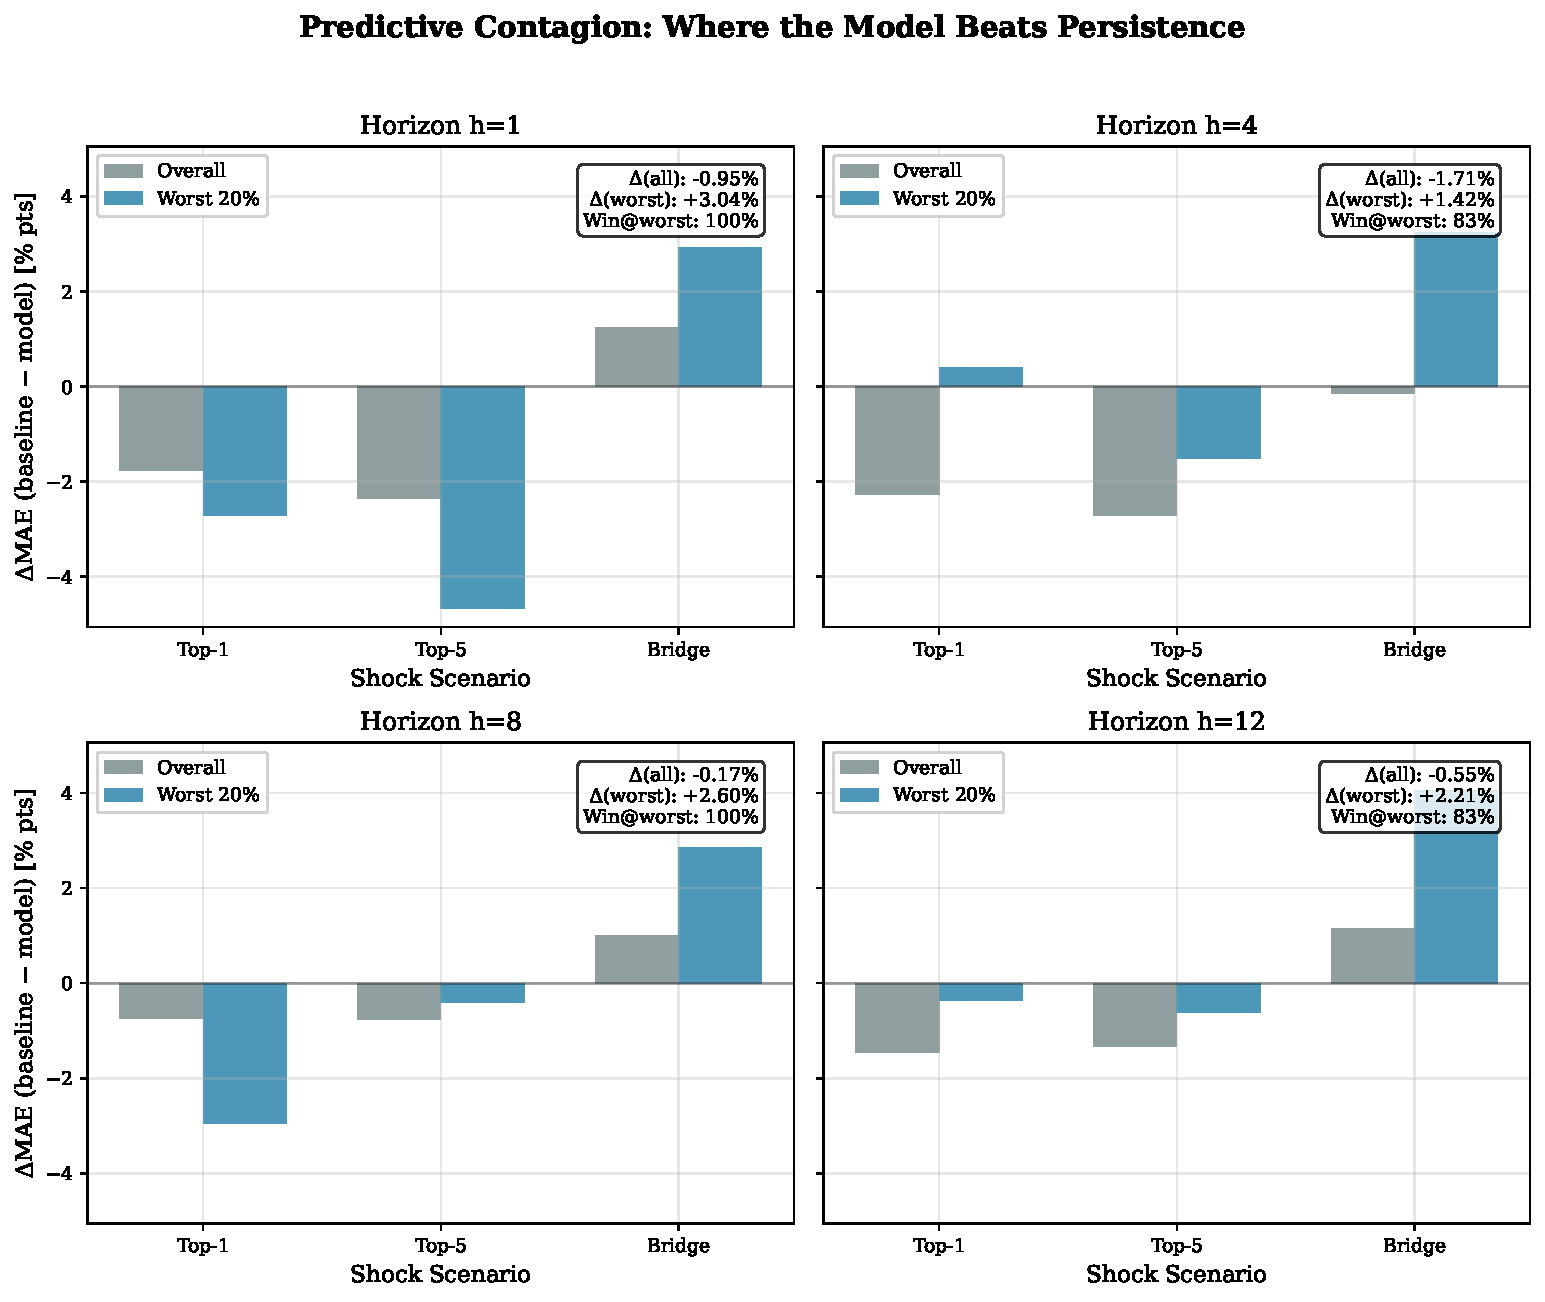
\includegraphics[width=0.95\textwidth]{figures/fig_contagion_advantage.pdf}
\caption{Advantage regimes for forward-looking stress testing. Bars report $\Delta\mathrm{MAE}=\mathrm{MAE}(\text{baseline})-\mathrm{MAE}(\text{model})$ in system loss (\% points). ``Overall'' is the full test set; ``Worst 20\%'' restricts to the 20\% largest baseline errors (tail regime). Positive values indicate DeXposure-FM outperforms persistence, highlighting where a foundation model adds value under non-stationarity.}
\label{fig:contagion-advantage}
\end{figure}

\begin{table}[t]
\centering
\small
\setlength{\tabcolsep}{6pt}
\begin{tabular}{lccc}
\hline
Horizon $h$ & $\Delta\mathrm{MAE}(\text{all})$ & $\Delta\mathrm{MAE}(\text{worst20\%})$ & Win rate (worst20\%) \\
\hline
1  & $-0.95$ & $+3.04$ & 100\% \\
4  & $-1.71$ & $+1.42$ & 83\% \\
8  & $-0.17$ & $+2.60$ & 100\% \\
12 & $-0.55$ & $+2.21$ & 83\% \\
\hline
\end{tabular}
\caption{Predictive stress testing summary (2025 hold-out). $\Delta\mathrm{MAE}$ is measured in system-loss percentage points. Worst20\% selects the 20\% largest persistence-baseline errors within each horizon (pooled across shock scenarios). ``Win rate'' is the fraction of worst20\% cases where the model has lower absolute error than persistence.}
\label{tab:contagion-advantage}
\end{table}

\section{Financial Economics Tools and Experimental Verifications}
\label{sec:econ}

Section~\ref{sec:evaluation} establishes DeXposure-FM's predictive performance on machine learning benchmarks. We now translate those outputs into financial-economics tools and provide experimental verifications that connect the model's forecasts to macroprudential use cases.

\subsection{Macroprudential Applications}
\label{subsec:macro-applications}

DeXposure-FM generates several outputs directly relevant to macroprudential monitoring of decentralised financial infrastructure, addressing the data gaps highlighted by international standard-setters \citep{FSB2023,IOSCO2023DeFi}.

\subsubsection{Systemic Risk Measurement: SIS and Spillovers}
\label{subsubsec:systemic-risk}
\textbf{Implementation.}
We compute protocol-level and network-level indicators on each weekly exposure snapshot. For protocol $p$, the Systemic Importance Score (SIS) combines interconnectedness, exposure concentration, and scale:
\begin{equation}
\text{SIS}_p = \alpha \cdot \text{PageRank}_p + \beta \cdot \text{TailExposure}_p + \gamma \cdot \log(\text{TVL}_p),
\label{eq:sis}
\end{equation}
where $\text{TailExposure}_p$ is the share of $p$'s top-$k$ outgoing exposures (we use $k=5$), and $\alpha,\beta,\gamma$ are non-negative weights that sum to 1 (default $\alpha=\beta=\gamma=1/3$). In parallel, we aggregate edge weights into a sector-to-sector spillover matrix $\mathbf{S}\in\mathbb{R}^{K\times K}$ where $S_{ij}$ is total exposure from sector $i$ to $j$, and compute a scale-invariant spillover concentration index as the HHI of off-diagonal entries:
\begin{equation}
\text{SpilloverIndex} = \text{HHI}\left(\{S_{ij} : i \neq j\}\right).
\end{equation}
\textbf{Use case.}
These measures operationalise the network-theoretic insight that interconnectedness, not just size, determines systemic fragility \citep{Acemoglu2015SystemicRisk,GlassermanYoung2016Contagion}. Weekly SIS rankings help identify protocols whose distress would propagate broadly, while spillover monitoring highlights sector pairs that act as risk conduits (e.g., stablecoins and bridges) \citep{KosseEtAl2023Stablecoin,ESRB2025,DieboldYilmaz2012}.

\subsubsection{Stress Testing and Contagion Assessment}
\label{subsubsec:contagion}
\textbf{Implementation.}
We implement a DebtRank-style contagion simulation to assess systemic loss propagation, following the loss-allocation logic of \cite{EisenbergNoe2001} and \cite{BattistonEtAl2012DebtRank}. Given an initial shock to protocol $p_0$ with loss ratio $\delta_0$:
\begin{enumerate}
  \item \textbf{Initialize:} $\text{Loss}_{p_0} = \delta_0 \cdot \text{TVL}_{p_0}$.
  \item \textbf{Propagate:} When a distressed debtor $p$ has loss $\text{Loss}_p$, we allocate its loss to its creditors $q$ proportionally to their exposures $E_{qp}$:
  \begin{equation}
    \Delta \text{Loss}_q \;=\; \text{Loss}_p \cdot \frac{E_{qp}}{\sum_{q'} E_{q'p}}.
  \end{equation}
  \item \textbf{Iterate:} If $\text{Loss}_q > \tau \cdot \text{TVL}_q$ (distress threshold $\tau=0.1$), protocol $q$ becomes distressed and propagates losses to its creditors. Losses are capped at $\text{TVL}_q$.
  \item \textbf{Terminate:} When no new protocols become distressed.
\end{enumerate}
We report total system loss (as a percentage of total TVL), contagion depth (propagation rounds), and affected-protocol counts. The three stress scenarios used throughout are: top protocol shock (50\% TVL loss), top-5 protocols shock (30\%), and bridge sector shock (100\%).

\textbf{Empirical verification.}
Section~\ref{subsec:stability} evaluates \emph{forward-looking} stress testing: we run the same simulator on $G_t$ (persistence baseline), $\hat{G}_{t+h}$ (model forecast), and $G_{t+h}$ (realized future) and compare the resulting system losses. Although persistence is hard to beat on average due to high edge overlap, DeXposure-FM improves in the worst 20\% tail regime where persistence fails (Table~\ref{tab:contagion-advantage}), with gains concentrated in bridge-sector shocks (Figure~\ref{fig:contagion-advantage}). Operationally, this suggests using the foundation model as a \emph{backstop} for scenario analysis during non-stationary periods.

\subsubsection{Forward-looking Risk Metric Forecasting}
\label{subsubsec:forward-looking-risk}
\textbf{Implementation.}
Beyond stress testing, we can forecast aggregate stability indicators by first predicting a future exposure graph $\hat{G}_{t+h}$ and then computing deterministic risk metrics on it (e.g., TVL concentration, edge concentration, network density, spillover index, and summary statistics of SIS). We compare these predicted metrics to their realized counterparts on $G_{t+h}$ across the 2025 hold-out set.

\textbf{Empirical verification.}
Figure~\ref{fig:forward-risk-scatter} reports predicted vs.\ realized risk metrics for $h\in\{1,4,8,12\}$. As expected under strong network persistence, many aggregates are difficult to outperform with persistence-style baselines, but the forecasts remain useful for \emph{trend monitoring} and for triggering deeper scenario analysis when predicted metrics move sharply.

\begin{figure}[t]
\centering
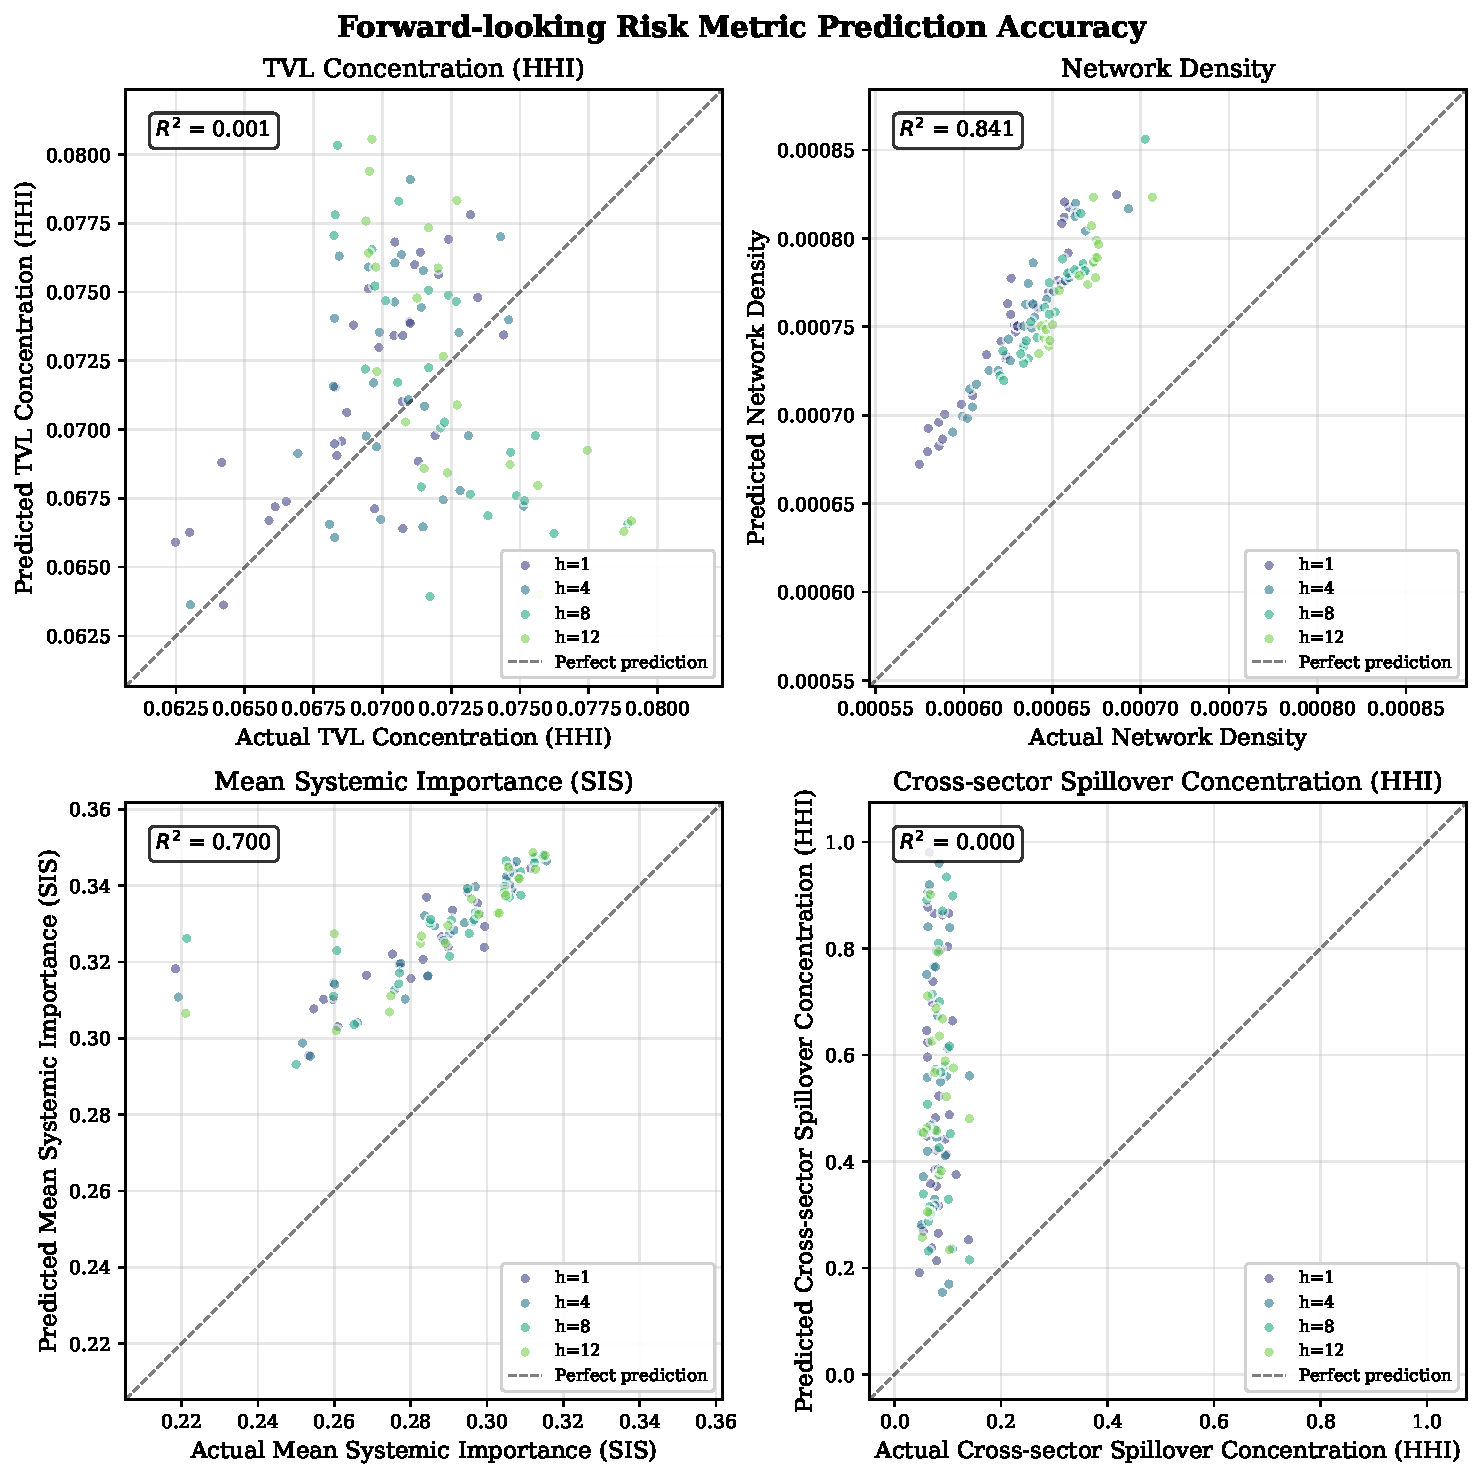
\includegraphics[width=0.95\textwidth]{figures/fig_forward_risk_scatter.pdf}
\caption{Forward-looking risk metric forecasting on predicted exposure graphs. Each point compares a realized metric on $G_{t+h}$ (x-axis) to the same metric computed on the predicted graph $\hat{G}_{t+h}$ (y-axis), across horizons.}
\label{fig:forward-risk-scatter}
\end{figure}

\subsubsection{Early Warning Signals and Event Studies}
\label{subsubsec:shock-events}
\textbf{Implementation.}
We examine two major stress events: the Terra/Luna collapse (May 9, 2022) and the FTX collapse (November 7, 2022). To avoid event leakage, for each event we train an event-specific forecaster using only snapshots strictly prior to the event window, then generate one-step-ahead forecasts within the event window. We track structural indicators and stress-test outcomes (via Section~\ref{subsubsec:contagion}) and monitor potential early warning features:
\begin{itemize}
  \item Density change: $\Delta\rho_t = (\rho_t - \rho_{t-1})/\rho_{t-1}$,
  \item Concentration spikes: $\Delta\text{HHI}_t > 2\sigma$,
  \item Assortativity shifts: rapid changes in degree correlation.
\end{itemize}

\textbf{Empirical verification.}
Table~\ref{tab:shock-results} summarizes structural shifts during the event windows, and Figure~\ref{fig:early-warning} compares predicted vs.\ realized trajectories for risk concentration and stress-test loss. These case studies illustrate how model-based forecasting can complement descriptive monitoring by providing forward-looking alerts around regime changes.

\begin{table}[t]
\centering
\small
\begin{tabular}{lcccc}
\hline
\textbf{Event} & \textbf{Pre-TVL (\$B)} & \textbf{Post-TVL (\$B)} & \textbf{$\Delta$TVL} & \textbf{$\Delta$Edges} \\
\hline
Terra/Luna & 257.1 & 171.0 & $-$33.5\% & +9.4\% \\
FTX & 127.0 & 177.2 & +39.5\% & $-$3.3\% \\
\hline
\end{tabular}
\caption{Network structure changes during stress events. Terra/Luna shows a classic flight-to-quality pattern with TVL collapse but edge count increase as capital reorganizes across protocols. The FTX event shows a \emph{positive} $\Delta$TVL because our dataset captures only on-chain DeFi protocols: the collapse of a centralised exchange triggered capital migration \emph{into} DeFi as users withdrew funds to self-custody, consistent with the ``flight to decentralisation'' narrative \citep{VidalTomasEtAl2023FTX}.}
\label{tab:shock-results}
\end{table}

\begin{figure}[t]
\centering
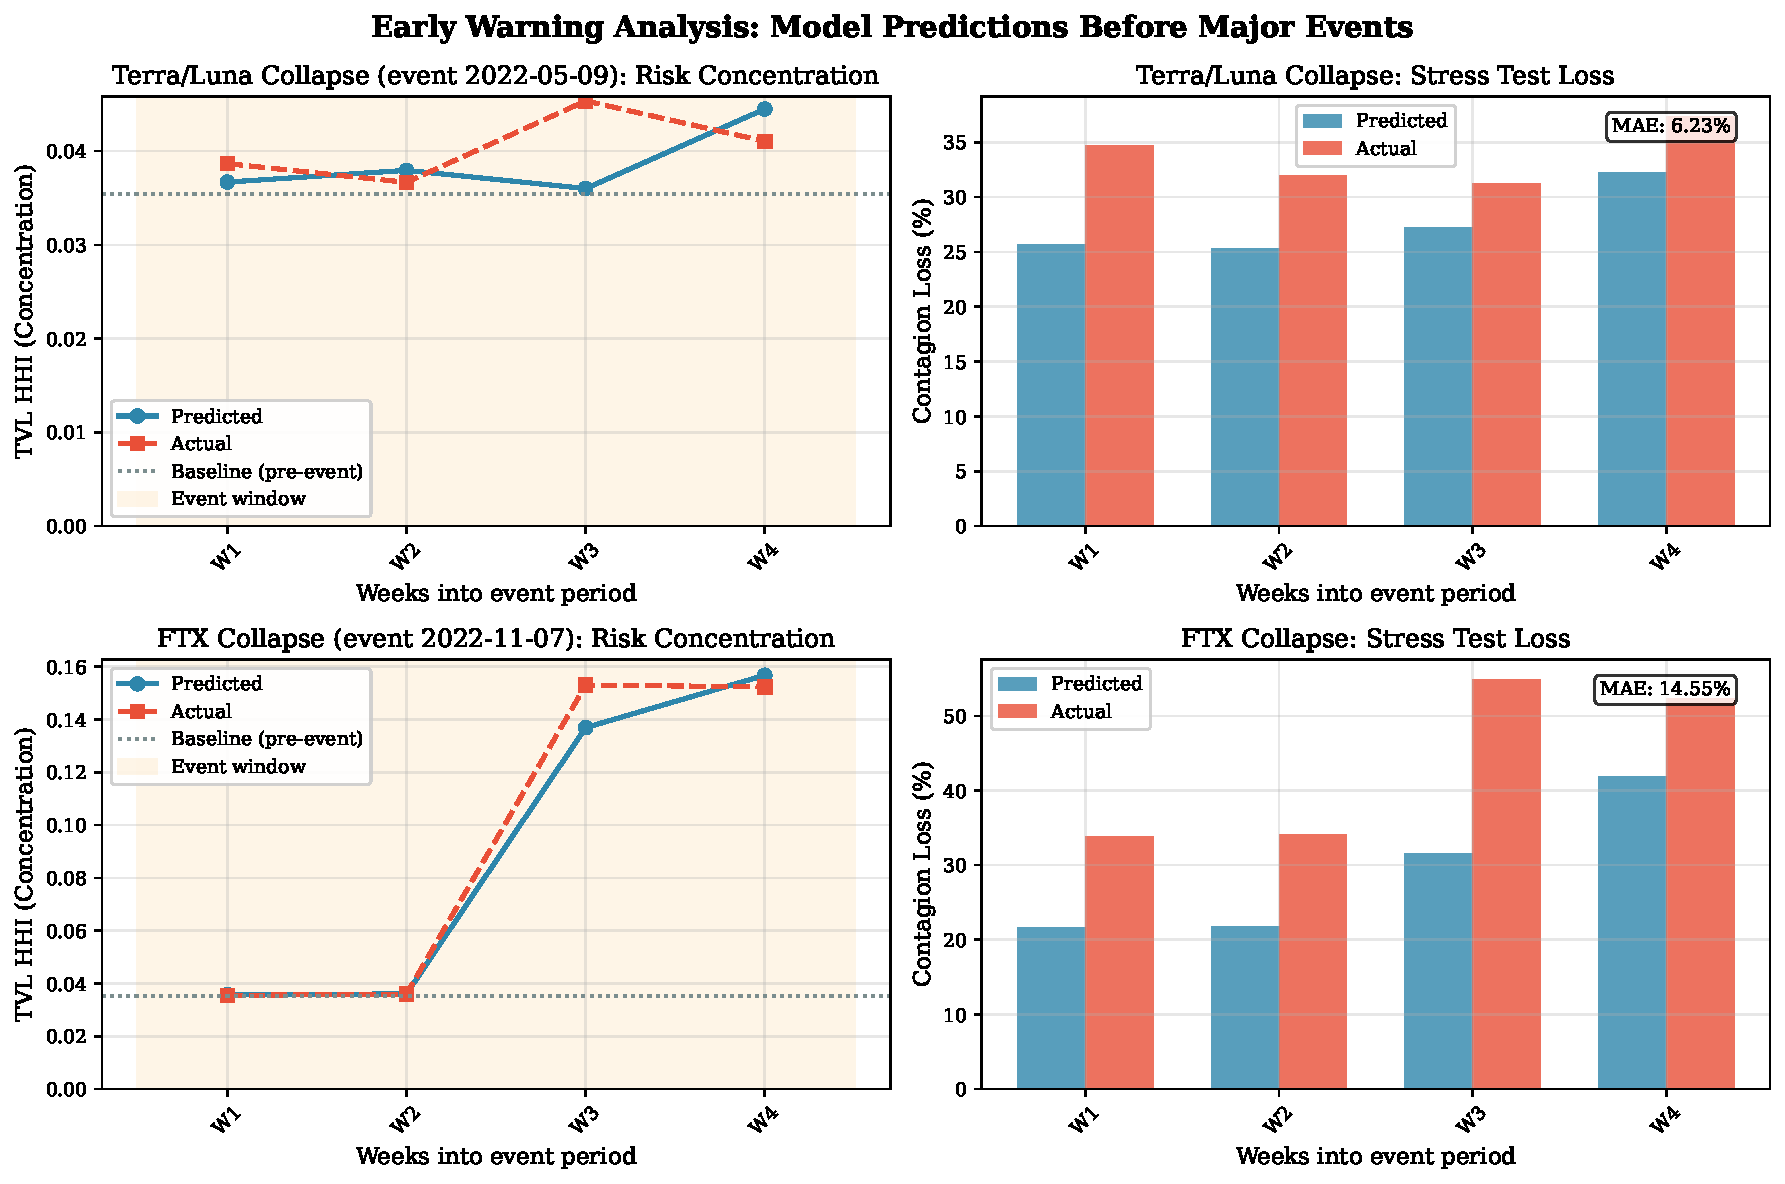
\includegraphics[width=0.95\textwidth]{figures/fig_early_warning.pdf}
\caption{Early warning event studies. For each event window, we compare predicted vs.\ realized risk concentration (HHI) and predictive stress-test loss (contagion system loss \%).}
\label{fig:early-warning}
\end{figure}


\subsection{Validity and Scope}
\label{subsec:validity}

Model-based risk measures are only as reliable as the conditions under which they were trained and validated \citep{MullainathanSpiess2017}. We identify several boundaries that users should keep in mind.

\paragraph{Stable versus turbulent regimes.}
The DeXposure dataset exhibits 98.5\% mean edge overlap week-to-week, meaning most credit relationships persist. Under such stable conditions, edge-existence forecasting is highly accurate (DeXposure-FM AUROC 0.993 at $h=12$; Table~\ref{tab:main-results}). During structural breaks---new protocol launches, governance attacks, or rapid deleveraging---the historical edge distribution may shift abruptly. In these regimes, persistence-style baselines can fail, and forward-looking models can add the most value (e.g., the worst20\% tail-regime gains in Table~\ref{tab:contagion-advantage}).

\paragraph{Coverage.}
DeXposure-FM is trained exclusively on on-chain DeFi protocols sourced from DeFiLlama. It does not observe:
\begin{itemize}
  \item Centralised exchange (CEX) balances or order-book exposures,
  \item Over-the-counter (OTC) derivatives or lending agreements,
  \item Off-chain reserves backing stablecoins (e.g., Treasury holdings of USDC) \citep{AnaduEtAl2023StablecoinsMMF}.
\end{itemize}
Consequently, the model captures intra-DeFi contagion but cannot directly assess spillovers to or from traditional financial institutions---a gap that matters as DeFi-TradFi linkages deepen \citep{ESRB2025}.

\paragraph{Temporal resolution.}
The dataset aggregates to weekly snapshots. Intraday or even daily dynamics---such as flash-loan attacks \citep{Qin2021FlashLoans} or rapid liquidation cascades \citep{Warmuz2023ToxicLiquidationSpirals}---are smoothed out. For high-frequency risk monitoring, complementary tools operating on block-level data would be required.


\subsection{Practical Caveats for Policymakers}
\label{subsec:caveats}

\paragraph{Complement, not replace, qualitative judgment.}
Model outputs such as SIS rankings and spillover indices are quantitative summaries, not definitive verdicts. A protocol may rank low on SIS yet pose idiosyncratic risks (e.g., smart-contract vulnerabilities, oracle manipulation) that network topology alone cannot capture \citep{DuleyEtAl2023Oracle,Gogol2024SoKDeFi}. Supervisors should triangulate model signals with code audits, governance analyses, and market intelligence.

\paragraph{TVL as a proxy for exposure.}
Total Value Locked is a convenient but imperfect measure \citep{Bertomeu2024}. It aggregates heterogeneous assets---stablecoins, volatile tokens, LP positions---without adjusting for liquidity or collateralisation quality. A protocol with \$1B in illiquid governance tokens is not equivalent to one with \$1B in USDC. Future work could incorporate asset-level risk weights to refine exposure estimates.

\paragraph{Model drift and retraining.}
DeFi evolves rapidly: new chains launch, token standards change, and incentive mechanisms shift. A model trained on 2020--2024 data may gradually lose accuracy as the ecosystem diverges from historical patterns. Periodic retraining on updated snapshots is essential to maintain forecast quality.

\paragraph{Cross-chain data consistency.}
DeXposure aggregates data across 602 blockchains, each with its own indexing quirks and oracle delays. Minor inconsistencies in timestamp alignment or token-price feeds can introduce noise. Users should be aware that edge weights near reporting boundaries may reflect data artefacts rather than genuine exposure changes.

\section{Future  Development Plan}

We plan to continuously update and improve DeXposure-FM. Below is our future development plan.

%\begin{itemize}
    %\item 
    
\subsection{Enlarging Training Data Pool} 
The current DeXposure-FM is trained on weekly inter-protocol snapshots from the DeXposure dataset, while leveraging pretrained TabPFN weights. While this provides broad on-chain coverage at a stable temporal resolution, it omits key off-chain channels through which DeFi is funded, hedged, and linked to traditional markets. In DeXposure-FM~2.0, we plan to expand the training pool by incorporating additional data sources, including centralized exchange (CEX) balances and order-book–implied exposures, over-the-counter (OTC) derivatives and lending agreements, and disclosures on off-chain stablecoin reserves (e.g., USDC’s Treasury-backed holdings). We also aim to add higher-frequency data (daily or intraday, where feasible), particularly around stress episodes, to better capture rapid deleveraging and liquidity dynamics that weekly aggregation smooths out.

\subsection{Expanding Proxies for Credit Exposure}
Total Value Locked (TVL) is a convenient but imperfect proxy for economic exposure. It aggregates heterogeneous assets into a single dollar value without adjusting for liquidity, haircuts, or collateral quality. As a result, equal TVL can imply very different loss-absorbing capacity and contagion risk; for example, \$1B held in thinly traded governance tokens is not economically equivalent to \$1B in USDC, and TVL can also move mechanically with prices even when underlying positions are unchanged. To address these limitations, DeXposure-FM~2.0 will incorporate asset-level risk weights and composition features (e.g., liquidity and volatility proxies, depeg risk, and observable collateral rules) to produce risk-adjusted exposure estimates and more interpretable systemic-risk indicators.

\subsection{Model Drift and Continuous Update}
DeFi evolves rapidly: new chains launch, token standards change, and incentive mechanisms shift. This non-stationarity implies that a model trained on historical regimes may gradually lose accuracy as exposures and flows depart from past patterns, including both gradual structural change and discrete breaks from major upgrades or new collateral rules. Periodic retraining on updated snapshots is therefore essential to maintain forecast quality, ideally paired with drift monitoring (e.g., calibration and error shifts by sector/chain) and versioned releases so that risk signals can be traced to specific data vintages and model iterations.

\subsection{Innovative Model Architecture}
The future DeXposure-FM 2.0 will include an innovative hybrid architecture that combines the current auto-regressive forecasting paradigm \citep{RasulEtAl2023LagLlama} with diffusion-based generative modeling \citep{MeijerChen2024DiffusionTS}. Auto-regressive models are efficient and accurate for point and conditional forecasts, but they can struggle to represent globally coherent network trajectories over long horizons, especially under stress. Diffusion models, by contrast, provide a principled way to learn complex conditional distributions by gradually denoising samples, and have recently shown strong performance in structured generation tasks, such as in diffusion language models \citep{LiEtAl2022DiffusionLM}. %In DeXposure-FM 2.0, we plan to use an autoregressive backbone to produce fast, state-dependent predictions of key sufficient statistics (e.g., protocol states and coarse exposure aggregates), while a conditional diffusion module refines these into full network realizations—jointly sampling link existence and weights in a way that preserves structural constraints such as sparsity, sectoral organization, and budget/flow consistency. This hybrid design would allow the model to output calibrated predictive distributions (not just point forecasts), support scenario-conditional stress testing via controlled guidance, and improve robustness to regime shifts by explicitly modeling the space of plausible future network configurations rather than committing early to a single trajectory.

\subsection{Open Source, Competitions, and Community Development}
We endeavor to develop DeXposure-FM to become fundamental infrastructure rather than a closed research artifact. We have released an open-source version of model weights and training code. We will continue our open-source efforts when improving the model. Based on the DeXposure dataset and DeXposure-FM model, we will organize public benchmarking competitions. These challenges will be designed to encourage robust methods and will include baseline implementations, leaderboards, and model cards reporting calibration and failure modes. We also aim to build a sustained community around DeFi economic measurement. By lowering barriers to entry and making the measurement process transparent, we hope to accelerate cumulative progress on reliable, policy-relevant tools for monitoring systemic risk in decentralized financial networks.



\section{Conclusions}
\label{sec:conclusion}

Credit exposures in decentralized finance (DeFi) are often embedded in token holdings and smart-contract interactions, rather than recorded as explicit bilateral claims, forming a tightly coupled network of inter-protocol dependencies. In such an environment, a disturbance to a single token can propagate across protocols, generating sizable and difficult-to-contain contagion. As DeFi becomes more intertwined with traditional financial infrastructure, most prominently via stablecoins, this evolving risk landscape calls for stronger tools to measure and forecast exposures. We introduce DeXposure-FM, which is arguably the first time-series, graph foundation model, designed for DeFi. DeXposure-FM combines a graph–tabular encoder with pretrained weights as initialization and multiple task-specific heads. It is trained on the DeXposure dataset, comprising 43.7 million observations spanning 4,300+ protocols on 602 blockchains and 24,300+ unique tokens. The model is trained for credit-exposure forecasting, jointly learning the dynamics of protocol-level flows, the evolving topology and weights of exposure links, and sectoral structure (e.g., lending, exchanges, asset management, bridges, stablecoins). Across a suite of machine-learning benchmarks, DeXposure-FM consistently outperforms strong competitors, including a prior graph foundation model and state-of-the-art temporal graph neural networks. We also translate the model outputs into economically interpretable indicators, including time-varying measures of systemic importance, sector-to-sector spillover indices, and early-warning signals based on shifts in network concentration and reliance on fragile collateral, which illustrate applications to macroprudential monitoring, DeFi stress testing, and counterfactual policy analysis. The tools are fully supported in he empirical validations. The model and code have been publicly available.


%DeXposure-FM demonstrates that graph foundation models can effectively measure and forecast inter-protocol credit exposures in decentralised finance. Trained on the DeXposure dataset spanning over 4,300 protocols across 602 blockchains from 2020 to 2025, the model learns joint representations of protocol-level dynamics, edge-level exposures, and sector structure. Evaluated on multi-step forecasting, historical stress-event analysis, and missing-edge imputation, GraphPFN-based variants maintain stable predictive performance (AUROC $>$0.91) across forecast horizons up to 14 weeks, outperforming temporal GNN baselines while prioritising economically significant edges.

%These predictive capabilities enable broader applications. DeXposure-FM provides a measurement layer for macroprudential monitoring: systemic importance scores, sector spillover matrices, and early-warning indicators derived from network structure. These outputs can support regulators in identifying concentration risks and conducting stress tests on DeFi infrastructure.

%While the current model is limited to on-chain DeFi data at weekly resolution, these constraints point toward promising extensions: integrating off-chain data sources to bridge DeFi and traditional finance, incorporating asset-level risk weights for finer exposure quantification, and scaling to real-time monitoring. As DeFi infrastructure continues to grow and interconnect with the broader financial system, we believe graph-based foundation models like DeXposure-FM can serve as a critical building block for cross-ecosystem risk surveillance.


%\section*{Acknowledgements}

%\bibliography{sections/DeXposure-FM}

%% The Appendices part is started with the command \appendix;
%% appendix sections are then done as normal sections
%\appendix




%% If you have bib database file and want bibtex to generate the
%% bibitems, please use
%%
\bibliographystyle{elsarticle-harv} 
\bibliography{sections/DeXposure-FM}

%% else use the following coding to input the bibitems directly in the
%% TeX file.

%% Refer following link for more details about bibliography and citations.
%% https://en.wikibooks.org/wiki/LaTeX/Bibliography_Management

%\begin{thebibliography}{00}

%% For numbered reference style
%% \bibitem{label}
%% Text of bibliographic item

%\bibitem{lamport94}
%  Leslie Lamport,
%  \textit{\LaTeX: a document preparation %system},
%  Addison Wesley, Massachusetts,
%  2nd edition,
%  1994.

%\end{thebibliography}



\end{document}

\endinput
%%
%% End of file `elsarticle-template-num.tex'.
